% !TEX program = pdflatex
% !TEX enableSynctex = true
\documentclass[aspectratio=169,10pt]{beamer}

%%%%%%%%%%%%%%%
\usepackage{booktabs}
\usepackage{xspace}
\usepackage{ulem}
\usepackage{subfig}
\usepackage{graphicx}
\usepackage{xcolor}
\usepackage{multirow}
\usepackage[capitalise,noabbrev]{cleveref} 
\usepackage{datatool}
\usepackage{algorithm} 
\usepackage{algpseudocode} 
\usepackage{empheq}
\usepackage[many]{tcolorbox}
\usepackage[capitalise,noabbrev]{cleveref}
\usetheme[progressbar=frametitle,block=fill]{metropolis}

\newcommand{\themename}{\textbf{\textsc{metropolis}}\xspace}
\definecolor{emphcolorval}{rgb}{0.23,0.4,0.7}
\definecolor{highlightcolorval}{rgb}{1,0,0}
% Penn colors
\definecolor{PennRed}{RGB}{149, 0, 26}
\definecolor{PennBlue}{RGB}{1, 37, 110}

\setbeamercolor{frametitle}{bg=PennBlue}
\setbeamercolor{progress bar}{fg=PennBlue}
\setbeamercolor{math text}{fg=PennRed}

\setbeamercolor{block title}{fg=PennBlue}
\setbeamercolor{block body}{fg=PennBlue}

\setbeamercolor{block title example}{fg=PennBlue}
\setbeamercolor{block body example}{fg=PennBlue, bg=yellow}

\setbeamersize{text margin left=5.5pt, text margin right=5.5pt}

\definecolor{cosmiclatte}{rgb}{1.0, 0.99, 0.95}
\setbeamercolor{background canvas}{bg=cosmiclatte}
%\titlegraphic{\hfill\includegraphics[height=0.8cm]{/Users/jesusfv/dropbox/Templates_Slides/penn_fulllogo.pdf}}
\newcommand{\emphcolor}[1]{\textbf{\textcolor{emphcolorval}{#1}}}
%\newcommand{\mathcolor}[1]{{\mathbf{\color{emphcolorval}{#1}}}}
\newcommand{\highlightcolor}[1]{{\textbf{\color{highlightcolorval}{#1}}}}

% \usepackage{natbib}
% \bibliographystyle{ecta}

\crefname{equation}{}{}
\newtheorem{proposition}{Proposition}
\newcommand\bigzero{\makebox(0,0){\text{\huge0}}}
\newcommand{\D}[1][]{\ensuremath{\boldsymbol{\partial}_{#1}}}
\newcommand{\R}{\ensuremath{\mathbb{R}}}
\newcommand{\diff}{\ensuremath{\mathrm{d}}}
\newcommand{\ex}{\ensuremath{\mathrm{ex}}}
\newcommand{\set}[1]{\ensuremath{\left\{{#1}\right\}}}
\newcommand{\indicator}[1]{\ensuremath{\mathds{1}\left\{{#1}\right\}}}
\newcommand{\condexpec}[3][]{\ensuremath{\mathbb{E}_{#1}\left[{#2} \; \middle| \; {#3} \right]}}
\newcommand{\prob}[2][]{\ensuremath{\mathbb{P}_{#1}\left( {#2} \right)}}
\newcommand{\cprob}[2]{\ensuremath{\mathbb{P}\left( {#1}\left| {#2} \right. \right)}}
\newcommand{\condcov}[2]{\ensuremath{\mathrm{cov}\left({#1} \; \middle| \; {#2} \right)}}
\newcommand{\expec}[2][]{\ensuremath{\mathbb{E}_{{#1}}\left[ {#2} \right]}}
\newcommand{\bigO}[1]{\ensuremath{\mathcal{O}(#1)}}
\newcommand{\Xdom}{\mathcal{X}}
\newcommand{\Yrange}{\mathcal{Y}}
\newcommand{\Xtrain}{\mathcal{X}_{\mathrm{train}}}
\newcommand{\Xextr}{\mathcal{X}_{\mathrm{extr}}}
\newcommand{\Xhull}{\mathrm{Hull}(\Xtrain)}
\newcommand{\Xtest}{\mathcal{X}_{\mathrm{test}}}
\newcommand{\Ltest}{\ell_{\mathrm{test}}}
\newcommand{\F}{\mathcal{F}}
\newcommand{\Resid}{\mathcal{R}}
\newcommand{\st}{\textrm{s.t.}\,}

\begin{document}
\title{{\vspace{0.4in}\hspace{0.2in}\textcolor{PennBlue}{AI and Economics: Solution Methods}}}
\author{\hspace*{4 mm} Mahdi Ebrahimi Kahou\inst{1}}

\institute{ \inst{\bf \hspace{0.2in} -- } \and
	\inst{\hspace{0.2in}1}Bowdoin College}


\date{}

\maketitle

\section{\textcolor{PennBlue}{Mathematical Models: Motivation}}

\begin{frame}{Why mathematical models?}
	\begin{itemize}
		\item Where is this?
	\end{itemize}
	\begin{figure}[t!]
		\centering
		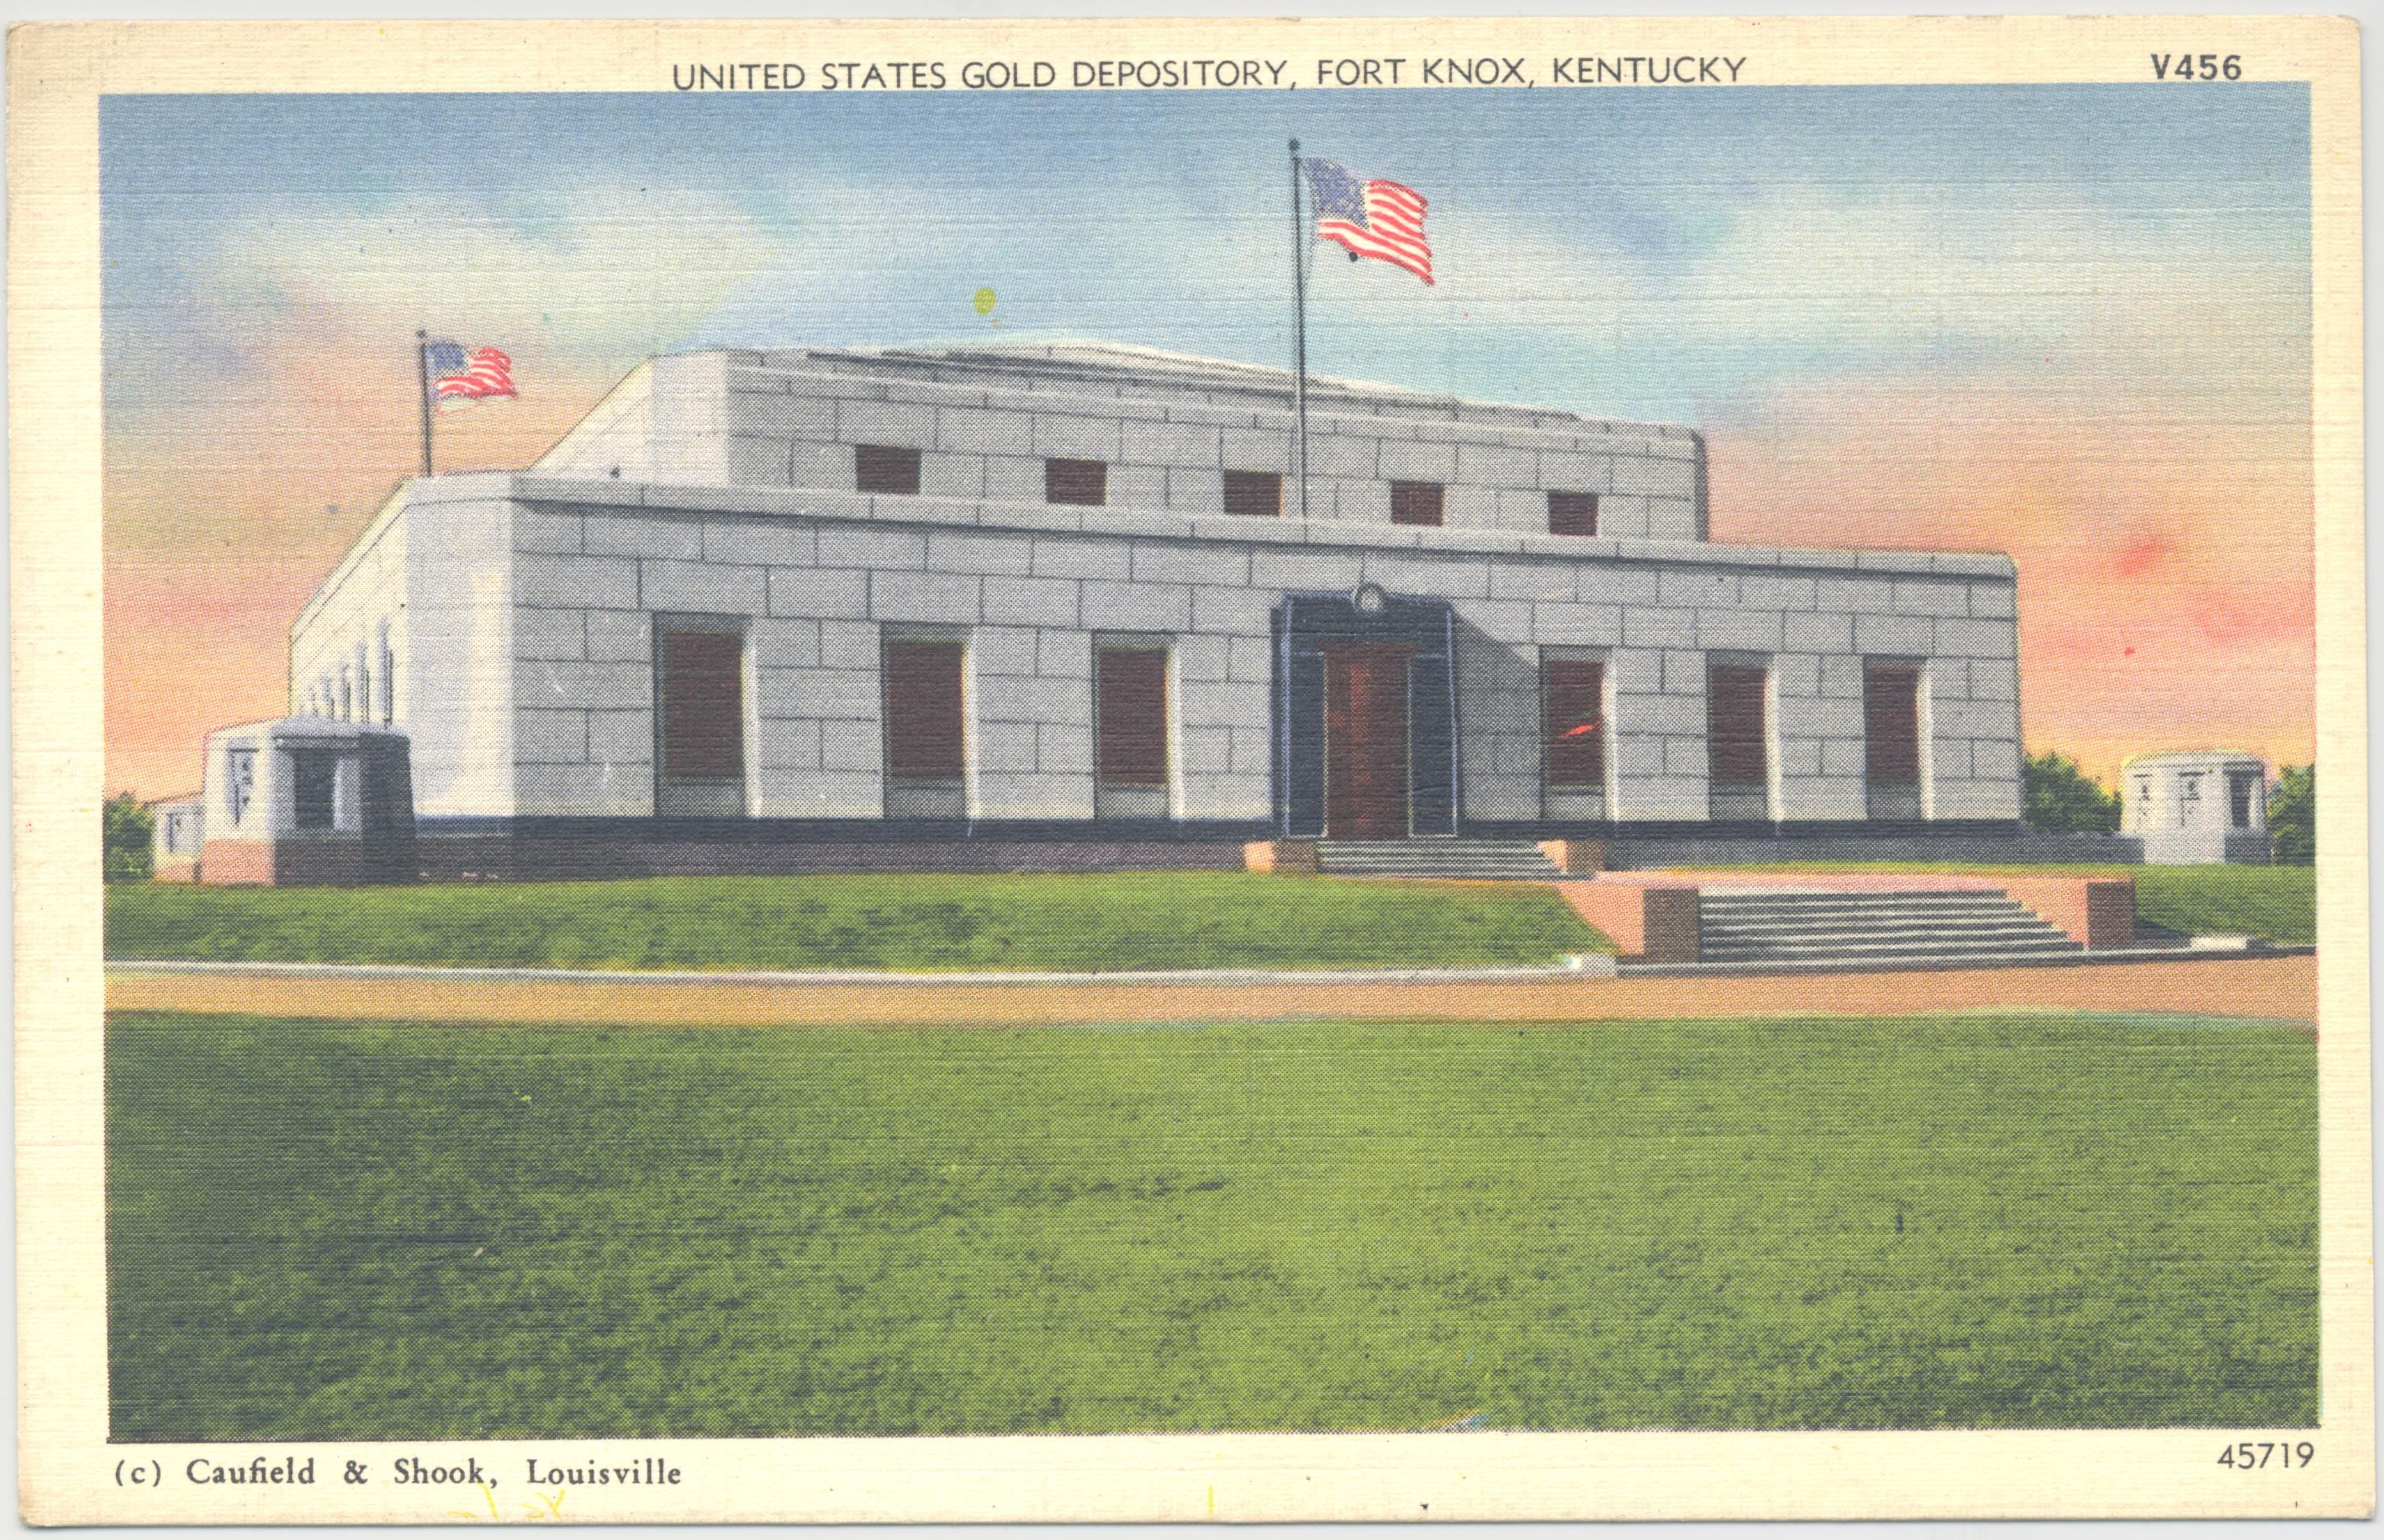
\includegraphics[width=0.65\textwidth]{figs/Fortknox}
	\end{figure}
\end{frame}

\begin{frame}{Why mathematical models?}
	\begin{itemize}
		\item Half a trillion dollars’ worth of gold.
	\end{itemize}
	\begin{figure}[t!]
		\centering
		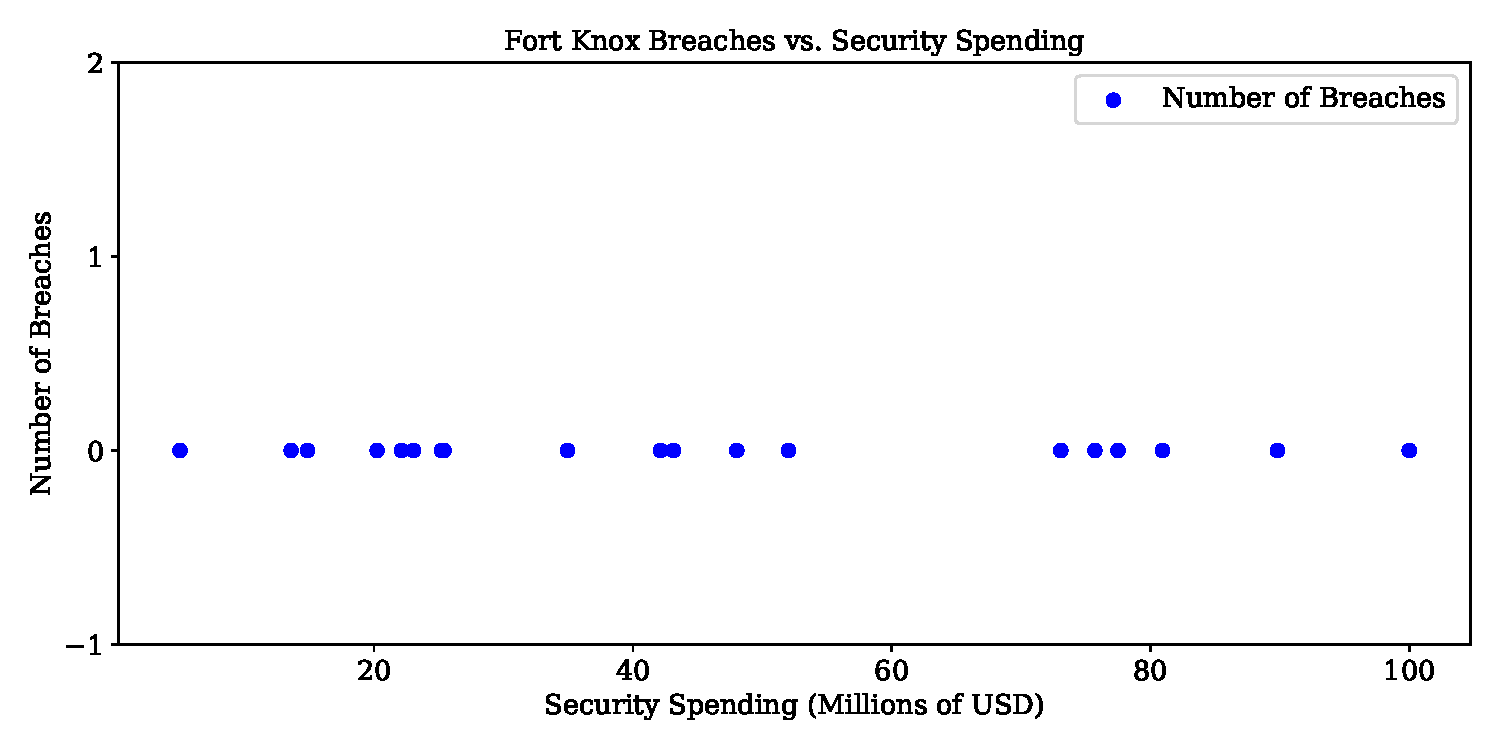
\includegraphics[width=0.65\textwidth]{figs/breaches}
	\end{figure}
	{\small Caution: The data on the $x$-axis is fictitious, but the $y$-axis data is accurate.}
\end{frame}

\begin{frame}{Why mathematical models?}
	\begin{itemize}
		\item \emphcolor{Policy Question}: \\
		By how much does decreasing the security budget by $70$ million dollars change the probability of a breach?
		\vspace{0.05in}
		\item How are you going to answer this?
		\vspace{0.05in}
		\item These are called \emphcolor{counterfactuals}.
	\end{itemize}
\end{frame}

\begin{frame}{Why mathematical models?}
	Scenarios similar to this:
	\begin{itemize}
		\item Predicting Economic Outcomes from Policy Changes:
		\begin{itemize}
			\item {\bf Scenario}: You want to understand the impact of a new tax policy on national income.
			\vspace{0.025in}
			\item {\bf Problem}: You cannot definitively assess how national income would have changed if the tax policy hadn't been implemented.
			\vspace{0.025in}
			\item {\bf Why} is it a problem? You need to know relationships between tax rates, consumer behavior, production, and other economic variables.
		\end{itemize}
	\end{itemize}
	
\end{frame}

\begin{frame}{Why mathematical models?}
	Scenarios similar to this:
	\begin{itemize}
		\item Evaluating the Impact of a Minimum Wage Increase on Employment:
		\begin{itemize}
			\item {\bf Scenario}: You want to determine how raising the minimum wage affects employment levels.
			\vspace{0.025in}
			\item {\bf Problem}: It's impossible to predict how different sectors or regions would be affected by the wage increase.
			\vspace{0.025in}
			\item {\bf Why} is it a problem? You need to know factors labor demand elasticity, substitution effects, or the interaction between wages and other economic variables.
		\end{itemize}
	\end{itemize}
	
\end{frame}


\begin{frame}{Why Mathematical Models?}
	\begin{quote}
		You cannot answer these questions without a (mathematical) \emphcolor{model}.	
	\end{quote}
	
	\begin{itemize}
		\item Model the incentives of the thieves, or their “payoff”.
		\vspace{0.025in}
		\item Model the incentives of the security team, and their decision-making process.
		\vspace{0.025in}
		\item Model the deterrence effects of security spending.
	\end{itemize}
\end{frame}

\begin{frame}{Why mathematical models?}
	Many of these problems are inherently \emphcolor{dynamic}. Consider the Fort Knox example:
	\begin{itemize}
		\item Technology improves over time.
		\vspace{0.025in}
		\item Fort Knox security planners anticipate that thieves will gain access to better technology in the future.
		\vspace{0.025in}
		\item Thieves, in turn, expect security measures (and spending) to increase in response.
	\end{itemize}
\end{frame}

\begin{frame}{Why Mathematical Models?}
	\begin{quote}
		Should we take our models \emphcolor{seriously}?
	\end{quote}
	\begin{itemize}
		\item When experiments are not feasible, modeling is your only option.
		\vspace{0.025in}
		\item Even when experiments are possible, causal inference alone doesn't reveal the mechanisms behind cause and effect.
	\end{itemize}
\end{frame}


\section{Economic Models}

\begin{frame}{Economic Models}
	 \begin{quote}
	 	If we have to take our models seriously what happens when they \emphcolor{dont} accept a \emphcolor{closed-form} solution?
	 \end{quote}
	 
	 \begin{itemize}
	 	\item Using numerical methods.
	 	\vspace{0.025in}
	 	\item Using the numerical solutions to study the counterfactuals.
	 \end{itemize}
	 
\end{frame}

\begin{frame}{Economic Models}
Problems with numerical methods in economics
	\begin{enumerate}
		\item They \emphcolor{fail} in complex and high-dimensional problems.
		\vspace{0.025in}
		\item The \emphcolor{dynamic} nature of the problem adds another layer of \emphcolor{complexity}.
	\end{enumerate}
\end{frame}

\begin{frame}{Economic Models and Recent Advances in Machine Learning}
		\begin{figure}[t!]
			\centering
			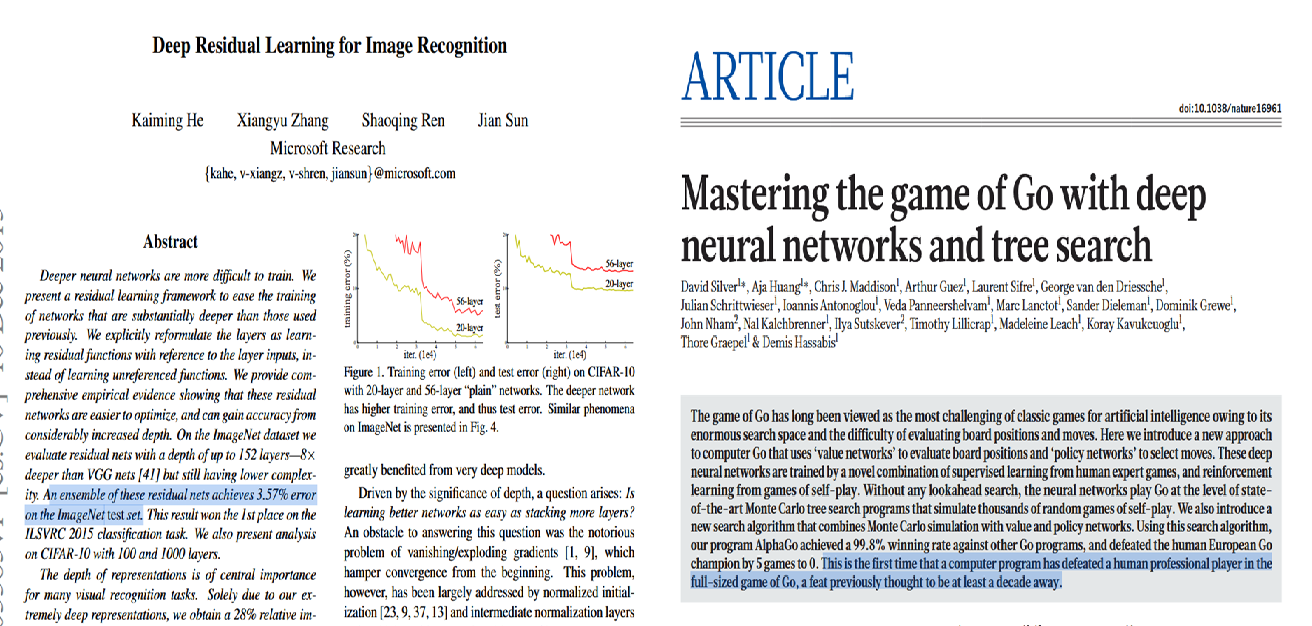
\includegraphics[width=0.7\textwidth]{figs/deep_learning}
		\end{figure}
\end{frame}


\begin{frame}{Economic Models and Machine Learning}
	Problems with numerical methods in economics
	\begin{enumerate}
		\item They \emphcolor{fail} in complex and high-dimensional problems.
		\vspace{0.025in}
		\begin{itemize}
			\item Recent advances in AI, promises in solving complex and high-dimensional problem. 
			\vspace{0.025in}
			\item Not going to talk about this today.
		\end{itemize}
		\vspace{0.025in}
		\item The \emphcolor{dynamic} nature of the problem adds another layer of \emphcolor{complexity}.
		\begin{itemize}
			\vspace{0.025in}
			\item Focus of the talk today.
		\end{itemize}
	\end{enumerate}
\end{frame}

\begin{frame}{Dynamic Models You Have Seen before}
	\begin{columns}
		\begin{column}{0.8\textwidth}
			% Content for the left column
			\begin{align*}
				\ddot{\theta}+ \omega^2 \sin(\theta) = 0
			\end{align*}
			\quad \quad \quad or 
			\begin{align*}
				\dot{\theta} &= \nu\\
				\dot{\nu} &= -\omega^2 \sin(\theta)
			\end{align*}
		\end{column}
		\begin{column}{0.2\textwidth}

		\end{column}
	\end{columns}
	%Four layer neural networks, with ReLU activation, 128 nodes
	%Four layer neural networks, with ReLU activation, 400 nodes
\end{frame}

\begin{frame}{Dynamic Models You Have Seen before}
	\begin{columns}
		\begin{column}{0.4\textwidth}
			% Content for the left column
			\begin{align*}
				\ddot{\theta}+ \omega^2 \sin(\theta) = 0
			\end{align*}
			\quad or 
			\begin{align*}
				\dot{\theta} &= \nu\\
				\dot{\nu} &= -\omega^2 \sin(\theta)
			\end{align*}
		\end{column}
		\begin{column}{0.6\textwidth}
			\begin{figure}[t!]
				\centering
				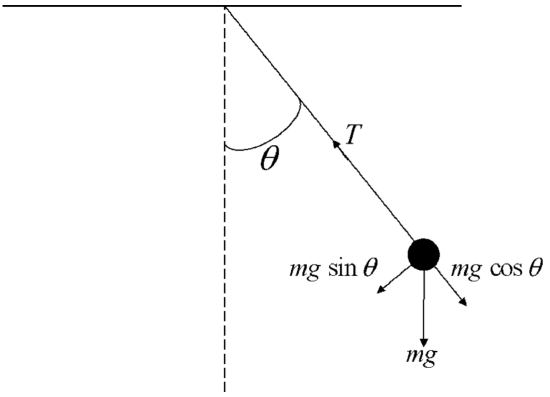
\includegraphics[width=\textwidth]{figs/pend}
				\vspace{-7mm}
			\end{figure}
		\end{column}
	\end{columns}
	%Four layer neural networks, with ReLU activation, 128 nodes
	%Four layer neural networks, with ReLU activation, 400 nodes
\end{frame}



	
\begin{frame}{Dynamic Models You Have Seen before}
	\begin{columns}
		\begin{column}{0.4\textwidth}
		A typical physicist to economists:
		\vspace{0.025in}
		\begin{itemize}
			\item “We solve problems like this every day.”
			\vspace{0.025in}
			\item “What’s all the fuss about?”
		\end{itemize}
		\end{column}
		\begin{column}{0.4\textwidth}
			\begin{figure}[t!]
				\centering
				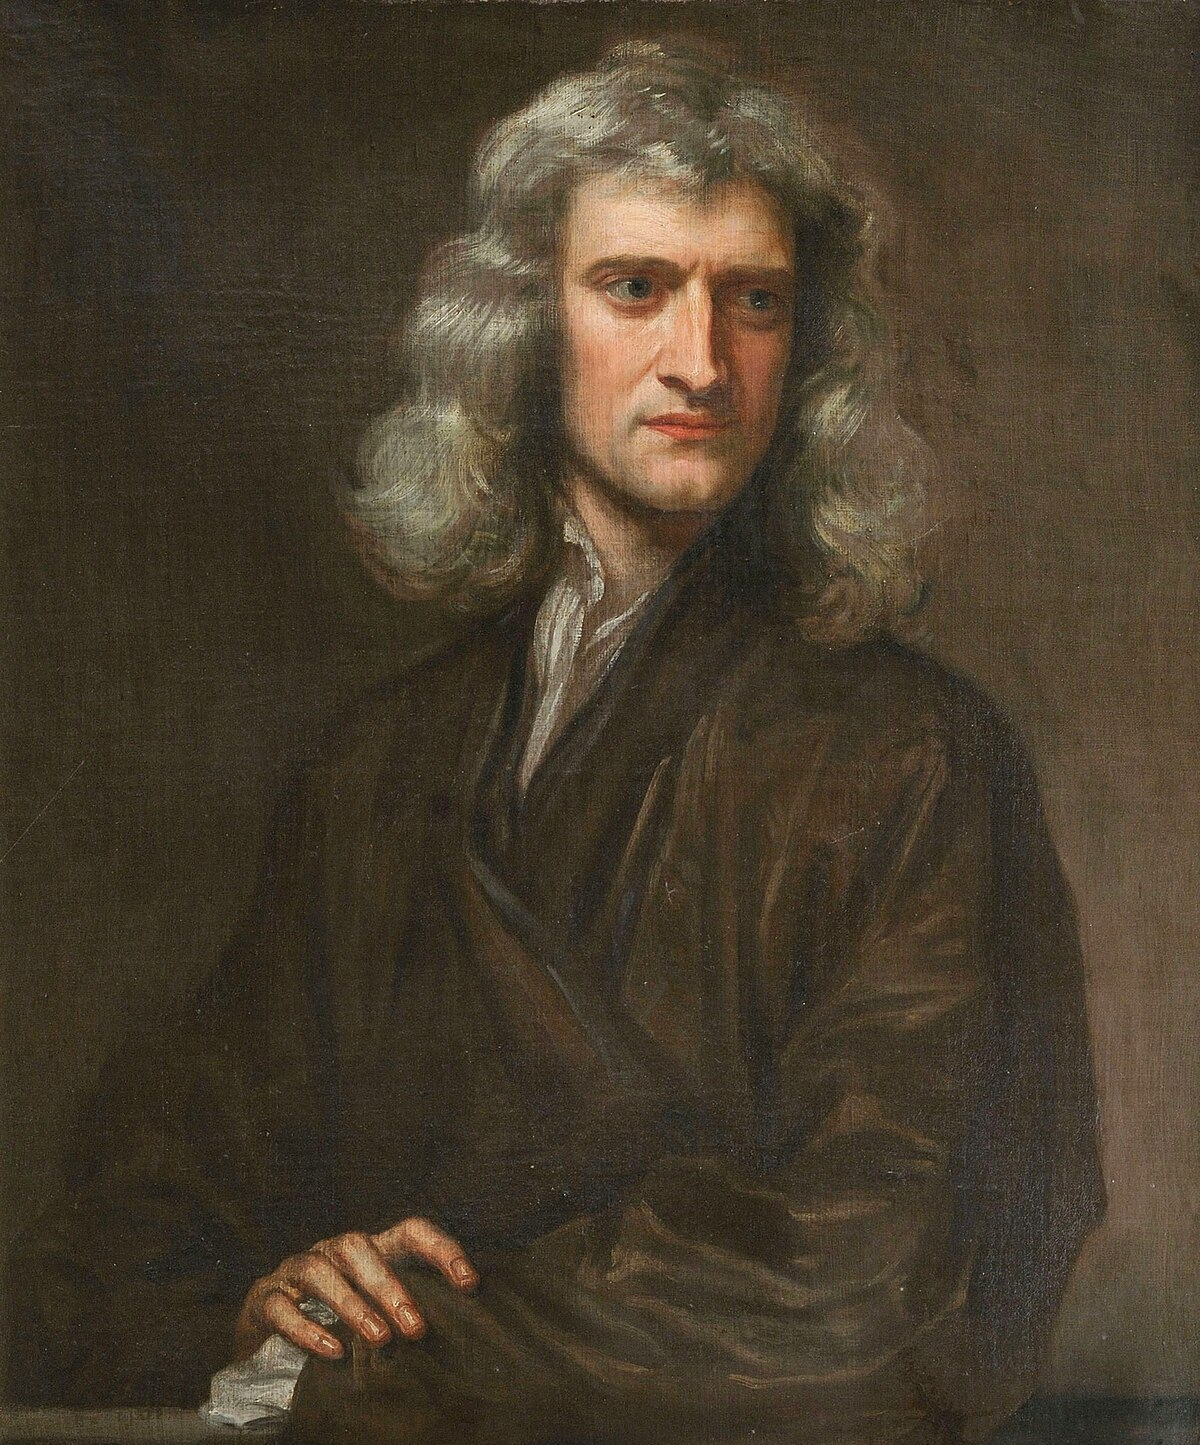
\includegraphics[width=\textwidth]{figs/newton}
				\vspace{-7mm}
			\end{figure}
		\end{column}
	\end{columns}
\end{frame}

\begin{frame}{Dynamic Models in Economics}
	\begin{columns}
		\begin{column}{0.4\textwidth}
		Dynamic models in Physics
			\begin{align*}
				x(t+1) &= f\left(x(t),y(t)\right)\\
				Y(t+1) &= g\left(x(t),y(t)\right)\\
				x(0)~&\text{is given}\\
				y(0)~&\text{is given}
			\end{align*}
			
		\end{column}
		\begin{column}{0.4\textwidth}
			Dynamic models in Economics
			\begin{align*}
				&x(t+1) = f\left(x(t),y(t)\right)\\
				&y(t+1) = g\left(x(t),y(t)\right)\\
				&x(0)~\text{is given}\\
				&\lim_{t\rightarrow\infty}h\left(x(t),y(t)\right) = 0
			\end{align*}
		\end{column}
	\end{columns}
	\begin{itemize}
		\item $\lim_{t\rightarrow\infty}h\left(x(t),y(t)\right) = 0$ is a \emphcolor{long-run} boundary condition.
	\end{itemize}
\end{frame}
	
\section{\textcolor{PennBlue}{Background: Economic Models, Deep learning and inductive bias}}


\begin{frame}
	\frametitle{Economic Models: functional equations}
	Many theoretical models can be written as functional equations:
	\begin{itemize}
		\item Economic object of interest: $f $, where $f : \Xdom\to \mathcal{R}\subseteq \mathbb{R}^N$ 
		\begin{itemize}
			\item e.g., asset price, investment choice, best-response, etc.
		\end{itemize}
			\vspace{0.1in}
		\item Domain of $f$: $\Xdom$  
		\begin{itemize}
			\item e.g. space of dividends, capital, opponents state or time in sequential models.
		\end{itemize}
			\vspace{0.1in}
		\item The ``Economics model'' error:  $\ell \big(x,f\big)$  
		\begin{itemize}
			\item e.g., Euler and Bellman residuals, equilibrium FOCs.
		\end{itemize}
		\vspace{0.1in}
	\end{itemize}
	Then a \emphcolor{solution} is $f^*\in \F$ where $\ell(x,f^*) = \mathbf{0}$ for all $x \in \Xdom$.\vspace{0.1in}
\end{frame}

%\begin{frame}
%	\frametitle{Example: one formulation of neoclassical growth}
%	An example of a recursive case:
%	\begin{itemize}
%		\item Domain: $x = \begin{bmatrix*}
%			k
%		\end{bmatrix*}
%		$ and $\Xdom = \R_+$.\vspace{0.1in}
%		\item Solve for the optimal policy $k'(\cdot)$ and consumption function $c(\cdot)$: So $\psi : \R \to \R^2$ and $\Yrange = \R^2_+$.\vspace{0.1in}
%		\item  Residuals are the Euler equation and feasibility condition, so $\Resid = \R^2$:
%		\begin{align*}
%			\ell(\underbrace{\begin{bmatrix*}k'(\cdot) & c(\cdot)\end{bmatrix*}}_{\equiv f}, \underbrace{k}_{\equiv x}) =
%			\underbrace{\begin{bmatrix*}
%					u'(c(k)) - \beta u'(c(k'(k)))\left(f'(k'(k)) + 1-\delta\right) \\
%					f(k) - c(k) - k'(k) + (1-\delta)k
%			\end{bmatrix*}}_{\text{model}}
%		\end{align*}
%		\item Finally,  $f^* = \left[k'(\cdot),c(\cdot)\right]$ is a solution if it has zero residuals on domain $\Xdom$.
%	\end{itemize}
%\end{frame}


\begin{frame}{Approximate solution: deep neural networks }
	\begin{enumerate}
		\item Sample $\mathcal{X}$: $\mathcal{D} = \{x_1,\cdots,x_N\}$
		\vspace{0.025in}
		\item Pick a family of parametric functions (e.g., deep neural networks) $f_\theta(\cdot) \in \mathcal{H}(\theta)$:
		\begin{itemize}
			\item $\theta$: parameters for optimization (i.e., weights and biases).  
		\end{itemize}
		\vspace{0.025in}
		\item To find an approximation for $f$ solve:
		\begin{align*}
			\min_{\theta } \frac{1}{N}\sum_{x \in \mathcal{D}} \|\underbrace{\ell(x,f_\theta)}_{\text{Econ model error}}\|_2^2
		\end{align*}
		\begin{itemize}
			\item Deep neural networks are highly over-parameterized: formally, $|\theta|\gg N$ 
		\end{itemize}
	\end{enumerate}
\end{frame}



\begin{frame}{Deep Neural Networks}
	\emphcolor{Deep learning} is \emphcolor{highly-overparameterized} $\mathcal{H}(\Theta)$ ($M\gg D$) class of functions.
	\begin{itemize}
		
		\item Example: one layer neural network, $f_{\theta} : \mathbb{R}^Q\rightarrow \mathbb{R}$:
		\begin{equation*}
			f_{\theta}(x) = W_2 \cdot \sigma \left(W_1\cdot x+b_1\right)+b_2
		\end{equation*}
		\vspace{0.1in}
		\item $W_1\in \mathbb{R}^{P\times Q}$, $b_1\in \mathbb{R}^{P\times 1}$, $W_2 \in \mathbb{R}^{1\times P}$, and $b_2 \in \mathbb{R}$.
		\vspace{0.1in} 
		\item $\theta \equiv \{b_1,W_1,b_2,W_2\}$ are the coefficients, in this example $M = PQ+P+P+1$.
		\vspace{0.1in} 
		\item $\sigma(\cdot)$ is a nonlinear function applied element-wise (e.g., $\max\{\cdot,0\}$).
		\vspace{0.1in}
		\item Making it ``deeper" by adding another ``layer":
		$f_{\theta}(x)\equiv W_3\cdot\sigma(W_2 \cdot \sigma(W_1 \cdot x + b_1) + b_2)+b_3.$
	\end{itemize}	
\end{frame}


\begin{frame}{Over-parameterized interpolation}
	\begin{itemize}
		\item Being over-parameterized ($|\theta|\gg N$), the optimization problem can have many solutions.
		\item Since individual $\theta$ are irrelevant it is helpful to think of optimization directly within $\mathcal{H}$
		\vspace{-0.025in}
		\begin{empheq}[box=\tcbhighmath]{equation*}
			\min_{f_{\theta} \in \mathcal{H}} \frac{1}{N}\sum_{x \in \mathcal{D}} \|\ell(x,f_{\theta})\|_2^2\label{eq:functional-optimization}
		\end{empheq}
		\vspace{-0.025in}
	\item But which $f_{\theta}$?
	\item \emphcolor{Mental model:} chooses min-norm interpolating solution for a (usually) unknown functional norm $\psi$
			\vspace{-0.025in}
	\begin{empheq}[box=\tcbhighmath]{align*}
		\min_{f_\theta\in \mathcal{H}} &||f_\theta||_\psi\\
		\st & \ell(x,f_\theta)=0,\quad \text{ for all } x \in \mathcal{D}
	\end{empheq}
	\vspace{-0.025in}
	\item That is what we mean by \emphcolor{inductive bias} (see Belkin, 2021 and Ma and Yang, 2021).
	
	\item  Characterizing $\psi$ (e.g., Sobolev norms or semi-norms?) is an active research area in ML.
	\end{itemize}
\end{frame}

\begin{frame}{Over-parameterization and smooth interpolation}
	\begin{itemize}
		\item Intuition: biased toward solutions which are flatter and have smaller derivatives
	\end{itemize}
		\begin{figure}[t!]
		\centering
		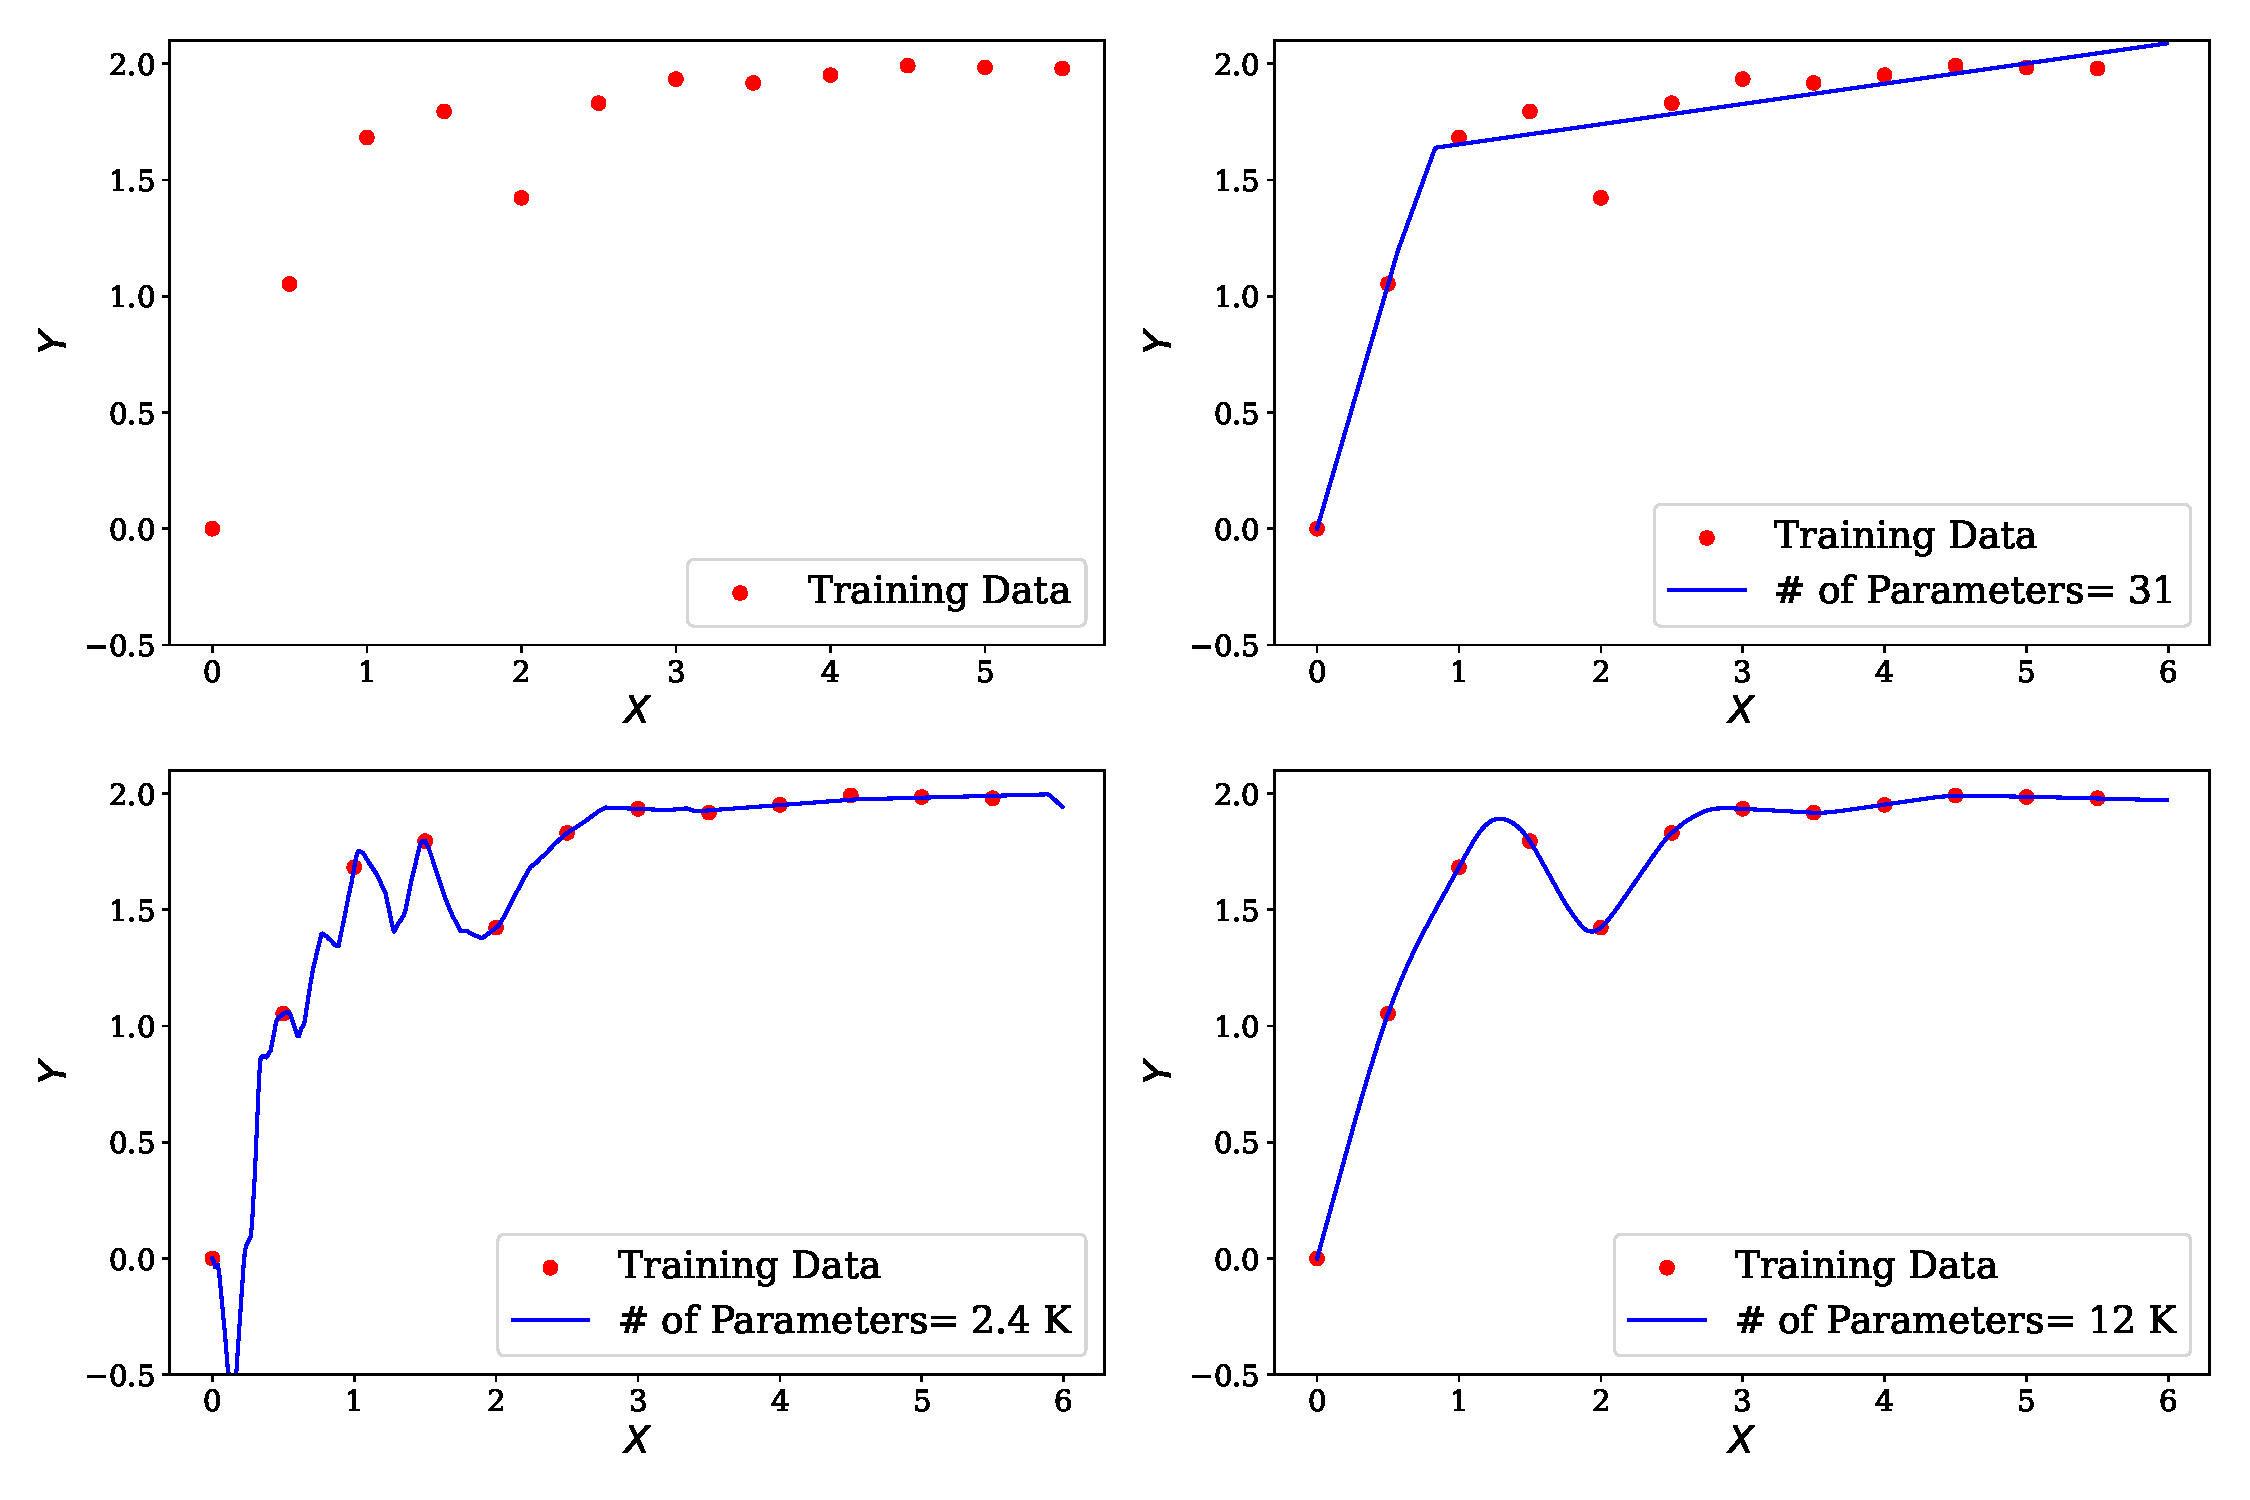
\includegraphics[width=0.65\textwidth]{figs/smooth_interpolation.pdf}
	\end{figure}
	%This is a one layer neural network
\end{frame}

\begin{frame}{Deep Learning: ``Fit Without Fear"?}
	\begin{columns}
		\begin{column}{0.4\textwidth}
			% Content for the left column
			\begin{itemize}
				\item ``{\it I remember my friend Johnny von Neumann used to say, with four parameters I can fit an elephant, and with five I can make him wiggle his trunk.}" \hfill Enrico Fermi
				\vspace{0.15in}
				\item {\it ``The best way to solve the problem from practical standpoint is you build a very big system ... basically you want to make sure you hit the zero training error" } \hfil Ruslan Salakhutdinov
			\end{itemize}
		\end{column}
		\begin{column}{0.6\textwidth}
			\begin{figure}[t!]
				\centering
				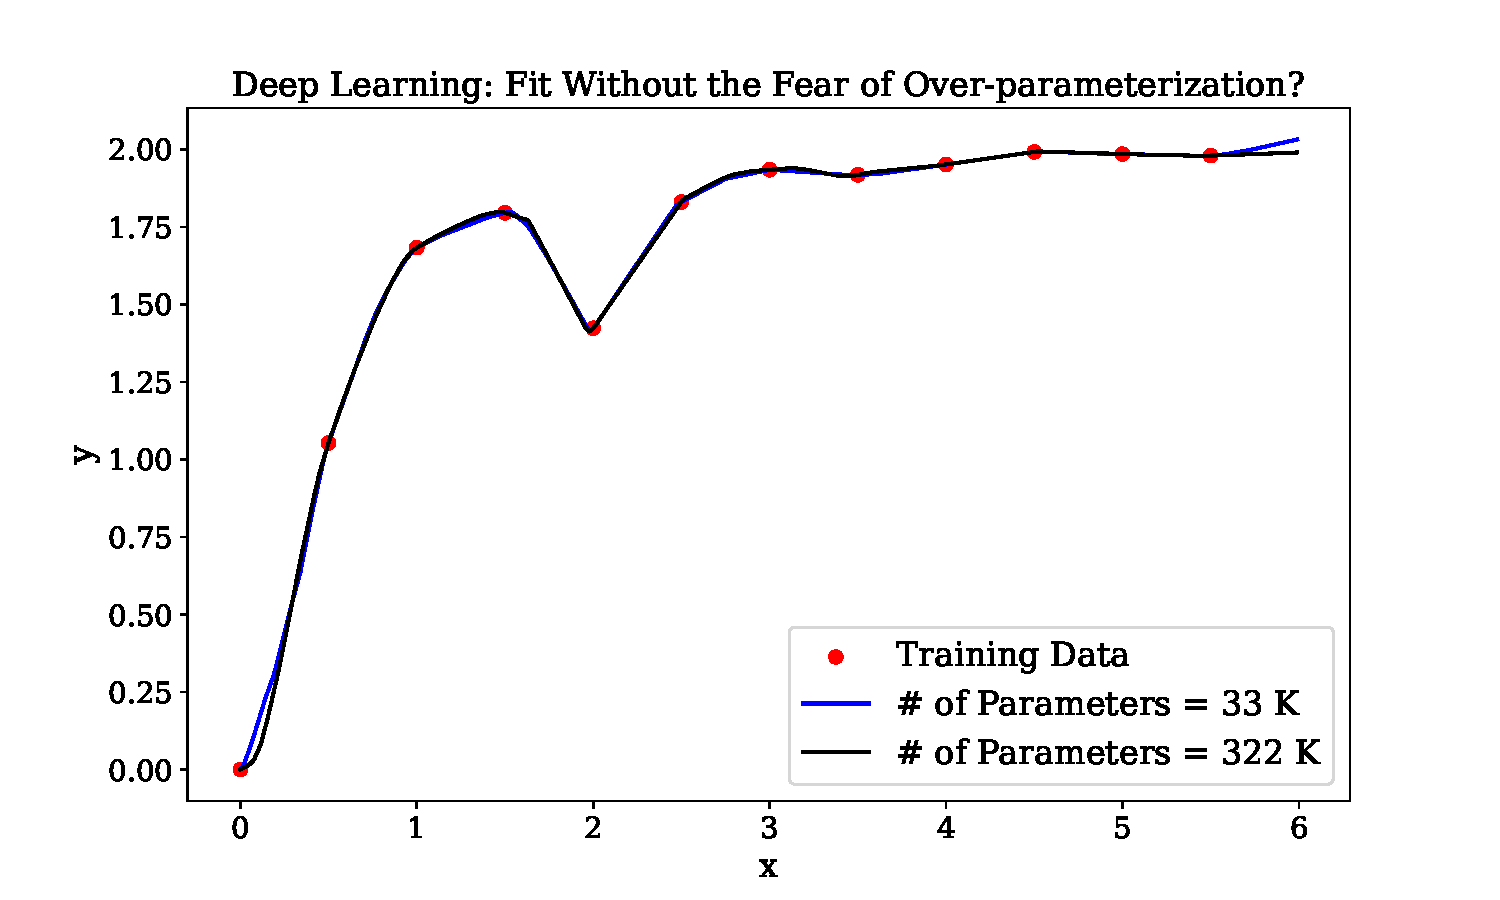
\includegraphics[width=\textwidth]{figs/smooth_interpolation_33_vs_322.pdf}
				\vspace{-7mm}
			\end{figure}
		\end{column}
	\end{columns}
	%Four layer neural networks, with ReLU activation, 128 nodes
	%Four layer neural networks, with ReLU activation, 400 nodes
\end{frame}


\begin{frame}{Deep Learning: random initialization and non-convex optimization  }
	\label{non_convex}
\vspace*{-1mm}

	\begin{figure}[t!]
		\centering
		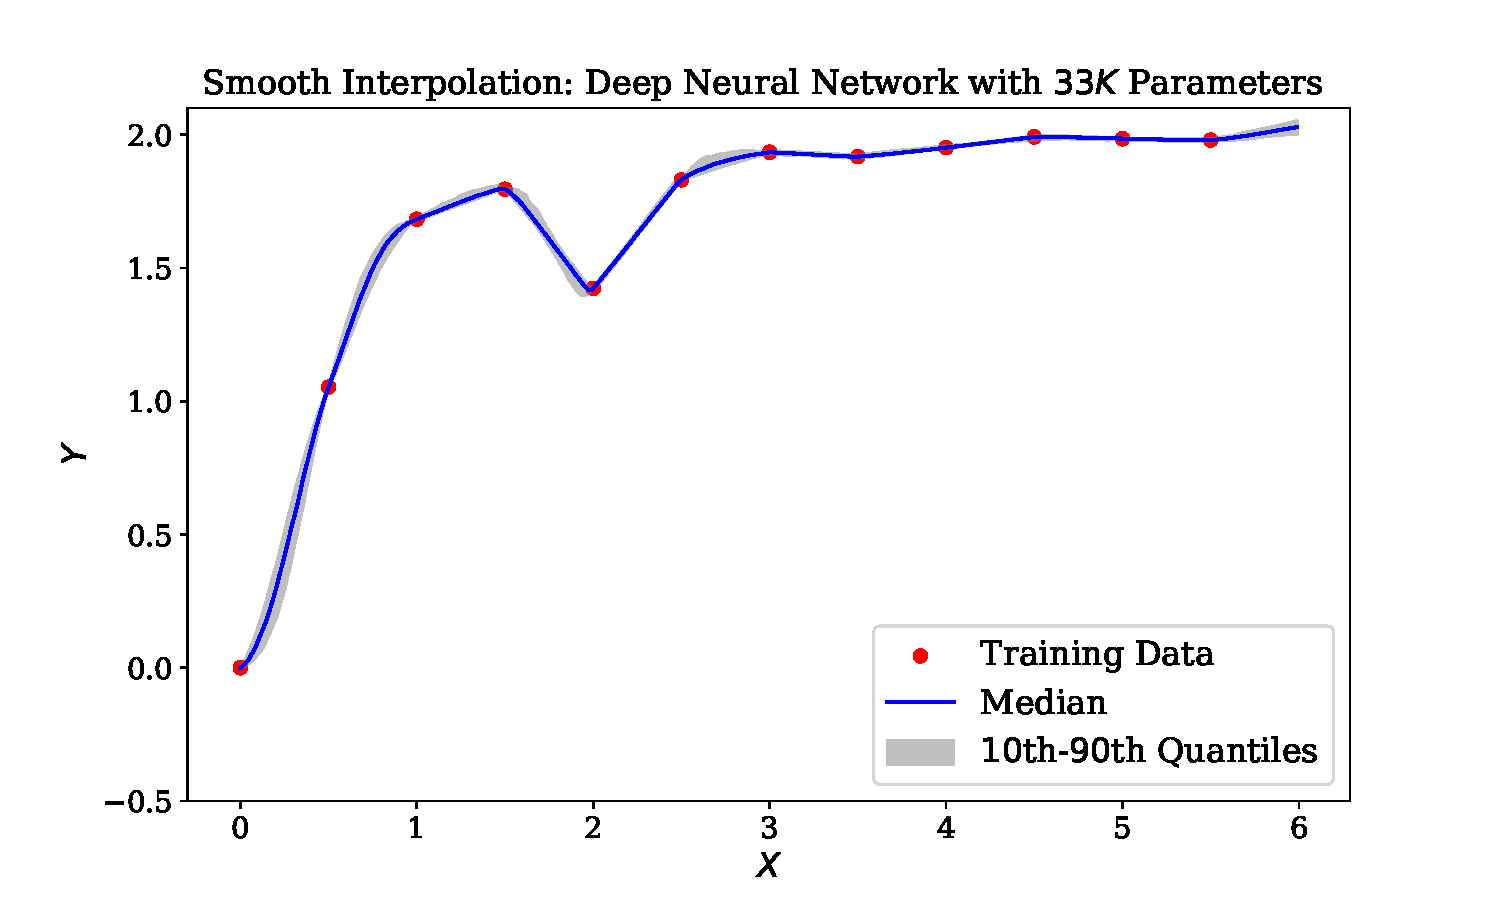
\includegraphics[width=0.75\textwidth]{figs/smooth_interpolation_100_seeds.pdf}
	\end{figure}
	%The parameters are irrelevant
	% RelU, 3 layers, Adam optimizer
	\hyperlink{dif_dist}{\beamerskipbutton{Different initialization}}
	%Four layer neural networks, with ReLU activation, 128 nodes
\end{frame}

\begin{frame}{Intuition of the paper}
	\begin{columns}
		\begin{column}{0.6\textwidth}
			% Content for the left column
			\begin{itemize}
				\item \emphcolor{Minimum-norm inductive bias}: 
				\begin{itemize}
					\item Over-parameterized models (e.g., large neural networks) interpolate the train data.
					%therefore they are many possible solutions
					\vspace{0.05in}
					\item They are biased towards interpolating functions with smaller norms. 
					\item So they dont like explosive functions.
				\end{itemize}
				\vspace{0.1in}
				\item \emphcolor{Violation of economic boundary conditions}:
				\begin{itemize}
					\item Sub-optimal solutions diverge (explode) over time.
					% As you can see in the plot optimal solution goe to the steady-state, the black dot, and any othe trajectory globaly or locally diveges. That is the signature of economic models
					\vspace{0.05in}
					% Given that they are divergent, then they are large functions with large norm
					\item This is due to the \emphcolor{saddle-path} nature of econ problems.
					% many economic models have this saddle path nature
					\vspace{0.05in}
					%\begin{itemize}
					%\item ``{\it Knife-edge stability is a common property of dynamic monetary models ...}" (Obstfeld and Rogoff, 1983).
					%\vspace{0.05in}
					%\end{itemize} 
					\item The long-run boundary conditions rule out the explosive solutions.
				\end{itemize}
			\end{itemize}
		\end{column}
		\begin{column}{0.4\textwidth}
		\begin{figure}[t!]
			\centering
			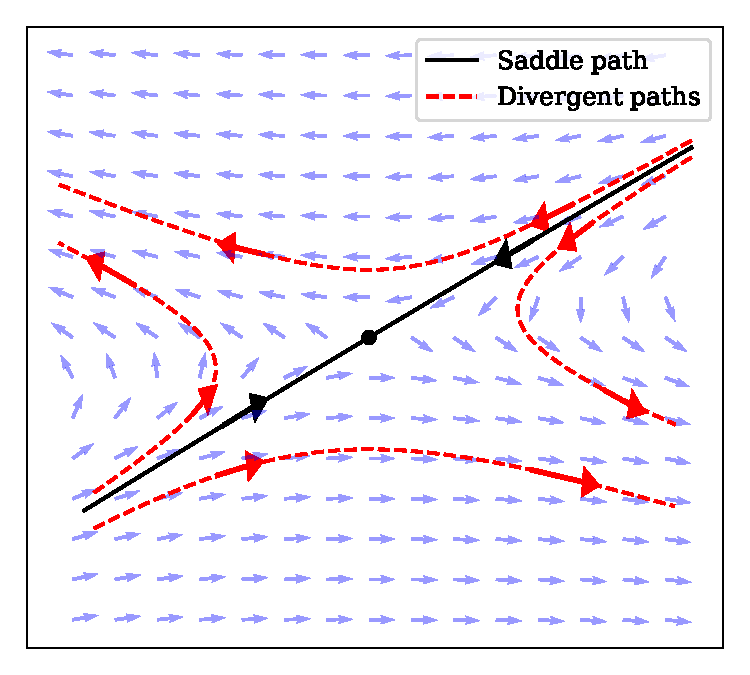
\includegraphics[width=\textwidth]{figs/saddle_path.pdf}
			\vspace{-7mm}
		\end{figure}
		\end{column}
	\end{columns}
\end{frame}

\section{Outline}

\begin{frame}{Outline of the talk}
	
	To explore how we can ignore the long-run boundary conditions, we show deep learning solutions to
	\begin{enumerate}
		\item Classic linear-asset pricing model.\vspace{0.1in}
		\item Sequential formulation of the neoclassical growth model.\vspace{0.1in}
		\item Sequential formulation of the neoclassical growth model with non-concave production function.\vspace{0.1in}
		\item Equivalent for a recursive formulation of the neoclassical growth model.\vspace{0.1in}
		
	\end{enumerate}
\end{frame}

\section{\textcolor{PennBlue}{Linear asset pricing and the no-bubble condition}}

\begin{frame}{Linear asset pricing: setup }
	\begin{itemize}
	\item The risk-neutral price, $p(t)$, of a claim to a stream of dividends, $y(t)$, is given by
	the recursive equation:
	\begin{align*}
		p(t) = y(t) + \beta p(t+1), \quad \text{for}~ t=0,1,\cdots
	\end{align*}
	\item $\beta<1$, and $y(t)$ is exogenous, $y(0)$ given.
	\item A two dimensional dynamical system with unknown initial condition  $p(0)$. This problem is \emphcolor{ill-posed}.
	\item A family of solutions
	 \begin{empheq}[box=\tcbhighmath]{align*}
	 	p(t) = \underbrace{p_f(t)}_{\text{fundamentals}} +  \underbrace{\zeta \left(\frac{1}{\beta}\right)^t}_{\text{explosive bubble}}
	 \end{empheq}
	 \item $p_f(t) \equiv \sum_{\tau =0}^\infty \beta^\tau y(t+\tau)$. Each solution corresponds to a different $\zeta>0$.
	\end{itemize}
\end{frame}


\begin{frame}{Linear asset pricing: the long-run boundary condition}
	\begin{columns}
		\begin{column}{0.5\textwidth}
			% Content for the left column
			\begin{itemize}
				\item Long-run boundary condition that rule out the explosive bubbles and chooses $\zeta =0$
				\begin{align*}
					\lim_{t\rightarrow \infty} \beta^t p(t) = 0.
				\end{align*}
				\vspace{0.1in}
				\item Any norm that preserve monotonicity, like $L_p$ and Sobolev (semi-)norms 
				\begin{align*}
					\min_{\zeta\geq 0} \|p\|_\psi = \|p_f\|_\psi
				\end{align*}
				\item Ignoring the no-bubble condition and using a deep neural network provides an accurate approximation for $p_f(t)$.
			\end{itemize}
		\end{column}
		\begin{column}{0.5\textwidth}
			\begin{figure}[t!]
				\centering
				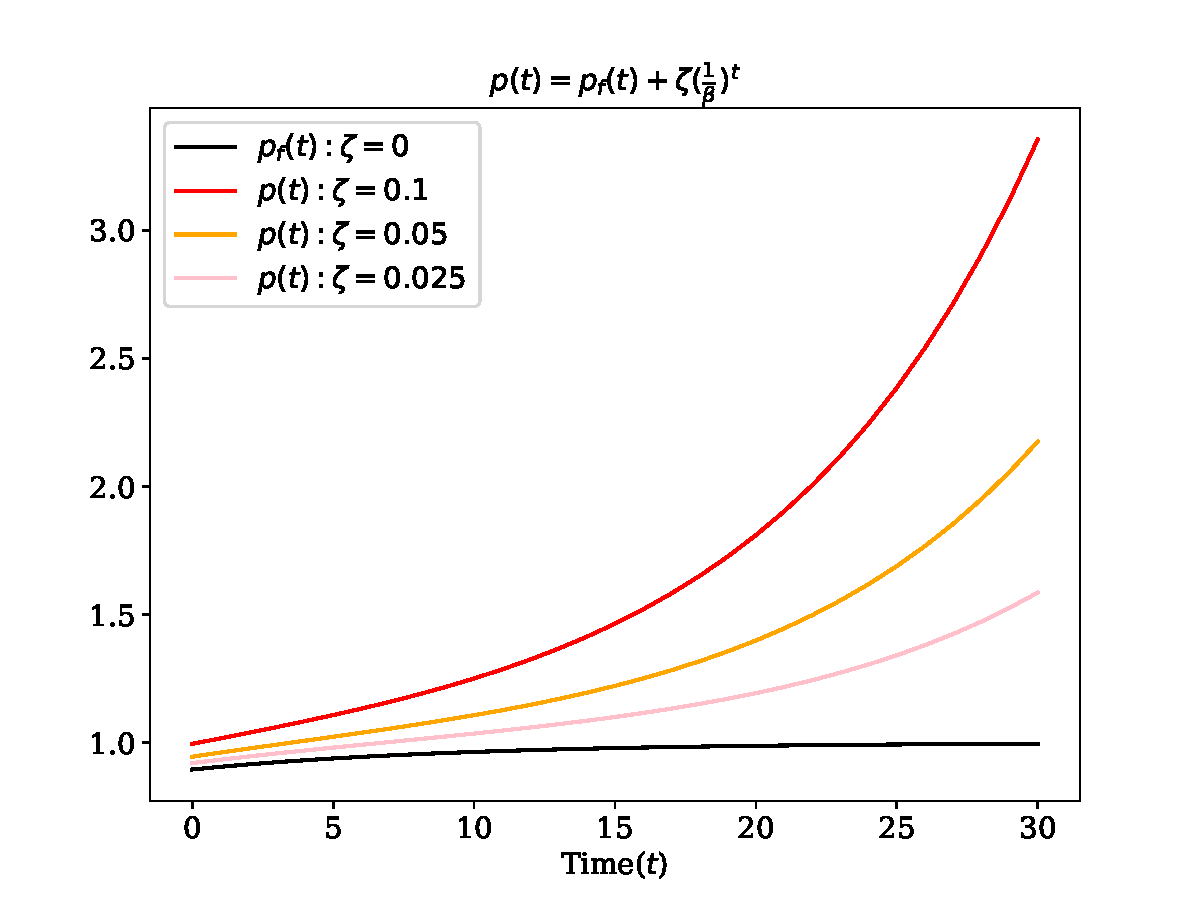
\includegraphics[width=\textwidth]{figs/bubble_solution.pdf}
				\vspace{-7mm}
			\end{figure}
		\end{column}
	\end{columns}
\end{frame}



\begin{frame}{Linear asset pricing: numerical method}
	\begin{itemize}
		\item Sample for time:  $\mathcal{D} = \{t_1,\cdots,t_N\}$.
		\item Generating the dividend process: $y(t+1) = c+(1+g)y(t)$, given $y(0)$.
		\item An over-parameterized neural network $p_\theta(t)$, \emphcolor{ignore} the non-bubble condition and solve 
				\begin{empheq}[box=\tcbhighmath]{align*}
				\min_{\theta} \frac{1}{N}\sum_{t \in \mathcal{D}} \left[p_\theta(t)- y(t)- \beta p_\theta(t+1)\right]^2
			\end{empheq}
		\item This minimization should provide an accurate short- and medium-run approximation for price based on the fundamentals $p_f(t)$.
	\end{itemize}
	
\end{frame}
\begin{frame}{Linear asset pricing: results}
	\begin{columns}
		\begin{column}{0.5\textwidth}
			% Content for the left column
			\begin{itemize}
				\item Two cases: $g<0$ and $g>0$.
				\vspace{0.05in}
				\item Relative errors: $\varepsilon_p(t)\equiv \frac{p_\theta(t)-p_f(t)}{p_f(t)}$.
				\vspace{0.05in}
				\item for $g>0$: $p_\theta(t) = e^{\phi t}
			 NN_\theta(t)$, $\phi$ is ``learnable".
			 	\vspace{0.05in}
				\item Results for $100$ different seeds (initialization of the parameters):
				\begin{itemize}
					\item important for \emphcolor{non-convex} optimizations.
				\end{itemize} 
				\vspace{0.05in}
				\item Very accurate short- and medium-run approximation.
			\end{itemize}
		\end{column}
		\begin{column}{0.5\textwidth}
			\begin{figure}[t!]
				\centering
				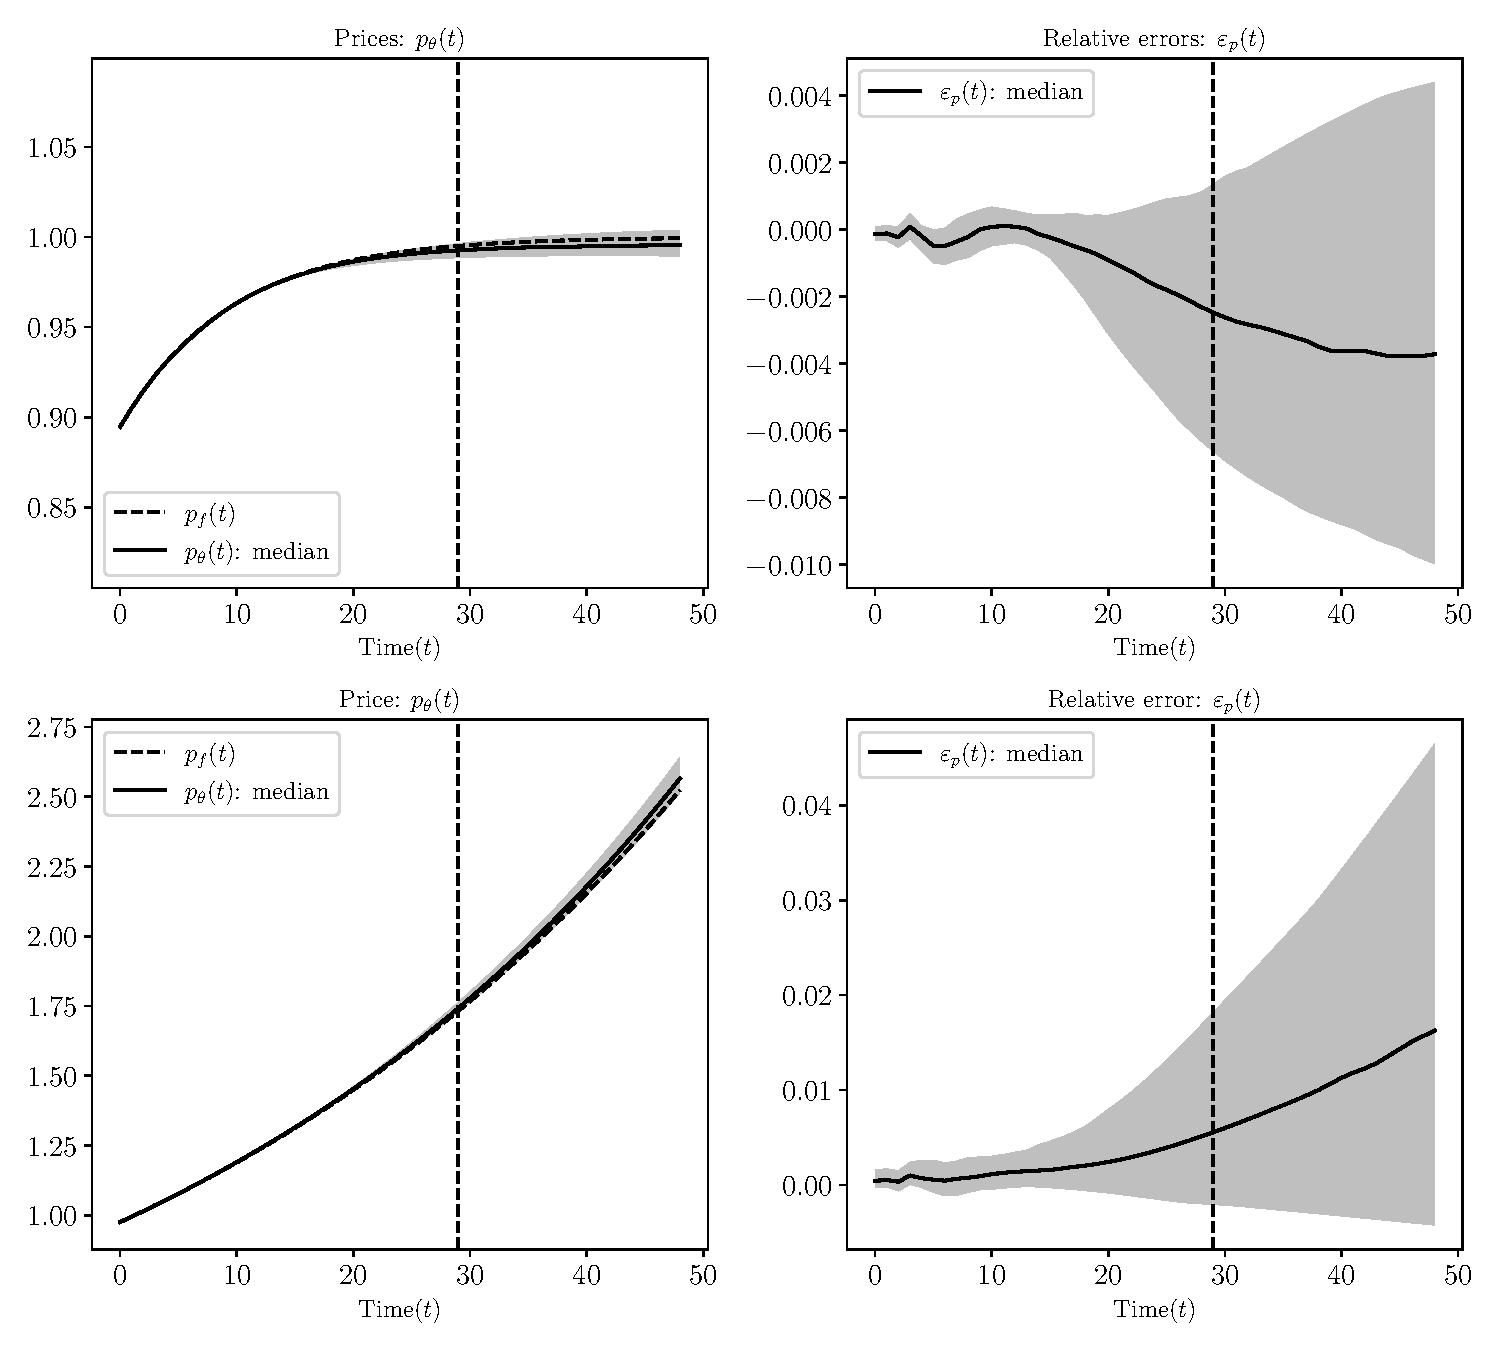
\includegraphics[width=\textwidth]{figs/asset_pricing_sequential_combined.pdf}
				\vspace{-7mm}
			\end{figure}
		\end{column}
	\end{columns}
\end{frame}



\begin{frame}[label= growing-dividends]{Learning the growth rate}
	
	\begin{figure}[htb]
		\centering
		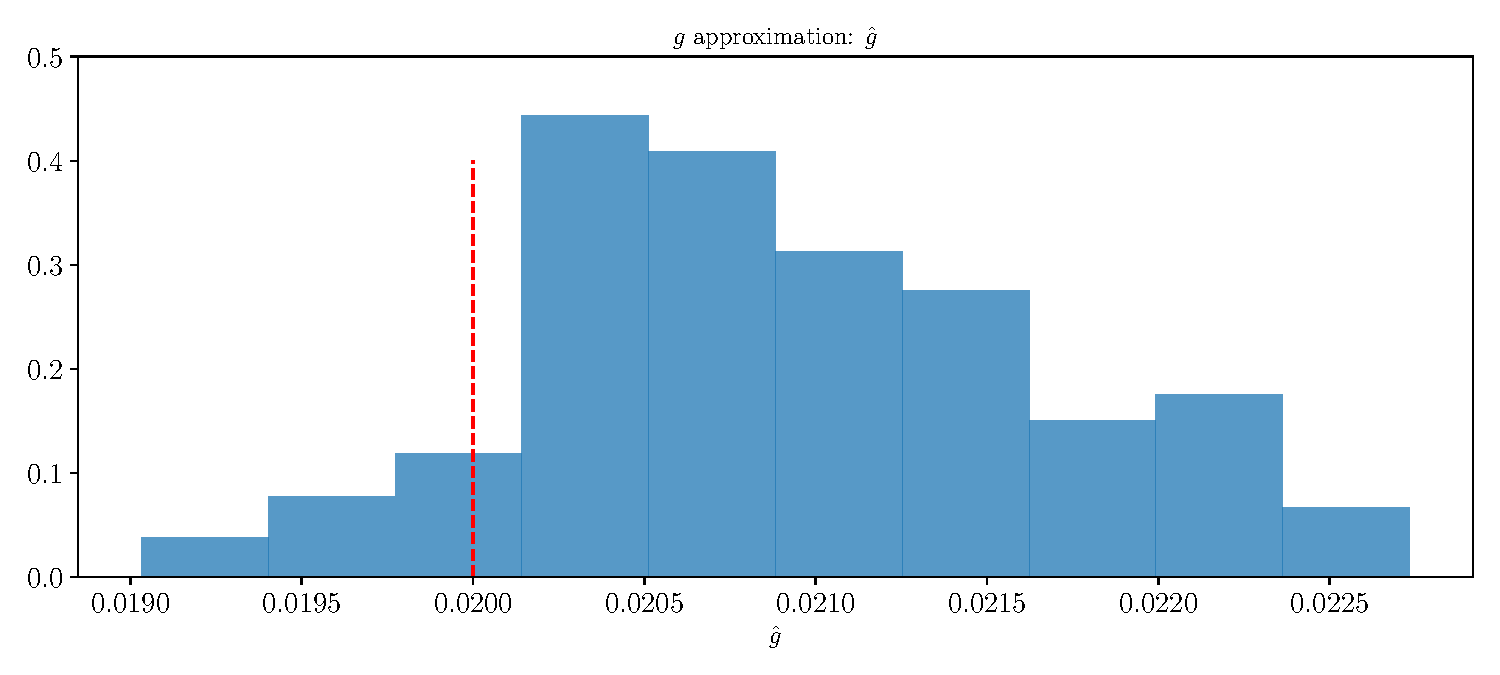
\includegraphics[width=9cm]{figs/asset_pricing_sequential_g_histogram.pdf}
	\end{figure}
	
	\begin{itemize}
		\item $\hat{g} = e^\phi -1$.
		\item Slightly biased due to small sample size, i.e., $\mathcal{D} = \{0,1,\cdots,29\}$.
	\end{itemize}

\end{frame}


\section{\textcolor{PennBlue}{Sequential neoclassical growth model and the transversality condition }}


\begin{frame}{Neoclassical growth model: setup }
	\begin{itemize}
		\item Total factor productivity $z(t)$ exogenously given, capital $k(t)$ with given $k(0)$, consumption $c(t)$, production function $f(\cdot)$, depreciation rate $\delta<1$, discount factor $\beta$  :
		\begin{align*}
			&\underbrace{k(t+1) = z(t)^{1-\alpha} f\left(k(t)\right)+ (1-\delta)k(t)-c(t)}_{\text{feasibility constraint}}, \\ 
			&\underbrace{c(t+1) = \beta c(t) \left[z(t+1)^{1-\alpha}f'\big(k(t+1)\big)+1-\delta\right]}_{\text{Euler equation}}.
		\end{align*}
	\item A three dimensional dynamical system with unknown initial condition  $c(0)$. This problem is \emphcolor{ill-posed}.
	\vspace{0.05in}
	\item A family of solutions, each solution corresponds to a different $c(0)$. Only one of them is the optimal solution.
	\end{itemize}	
\end{frame}

\begin{frame}{Neoclassical growth model: the long-run boundary condition}
	\begin{columns}
		\begin{column}{0.35\textwidth}
			% Content for the left column
			\begin{itemize}
				\item To rule out sub-optimal solutions, transversality condition
				\begin{align*}
					\lim_{t\rightarrow \infty}\beta^t \frac{k(t+1)}{c(t)} = 0.
				\end{align*}
				\vspace{0.1in}
				\item  Using a deep neural network and ignoring the transversality condition provides a an accurate approximation for the optimal capital path.
			\end{itemize}
		\end{column}
		\begin{column}{0.7\textwidth}
			\vspace{-10mm}
			\begin{figure}[t!]
				\centering
				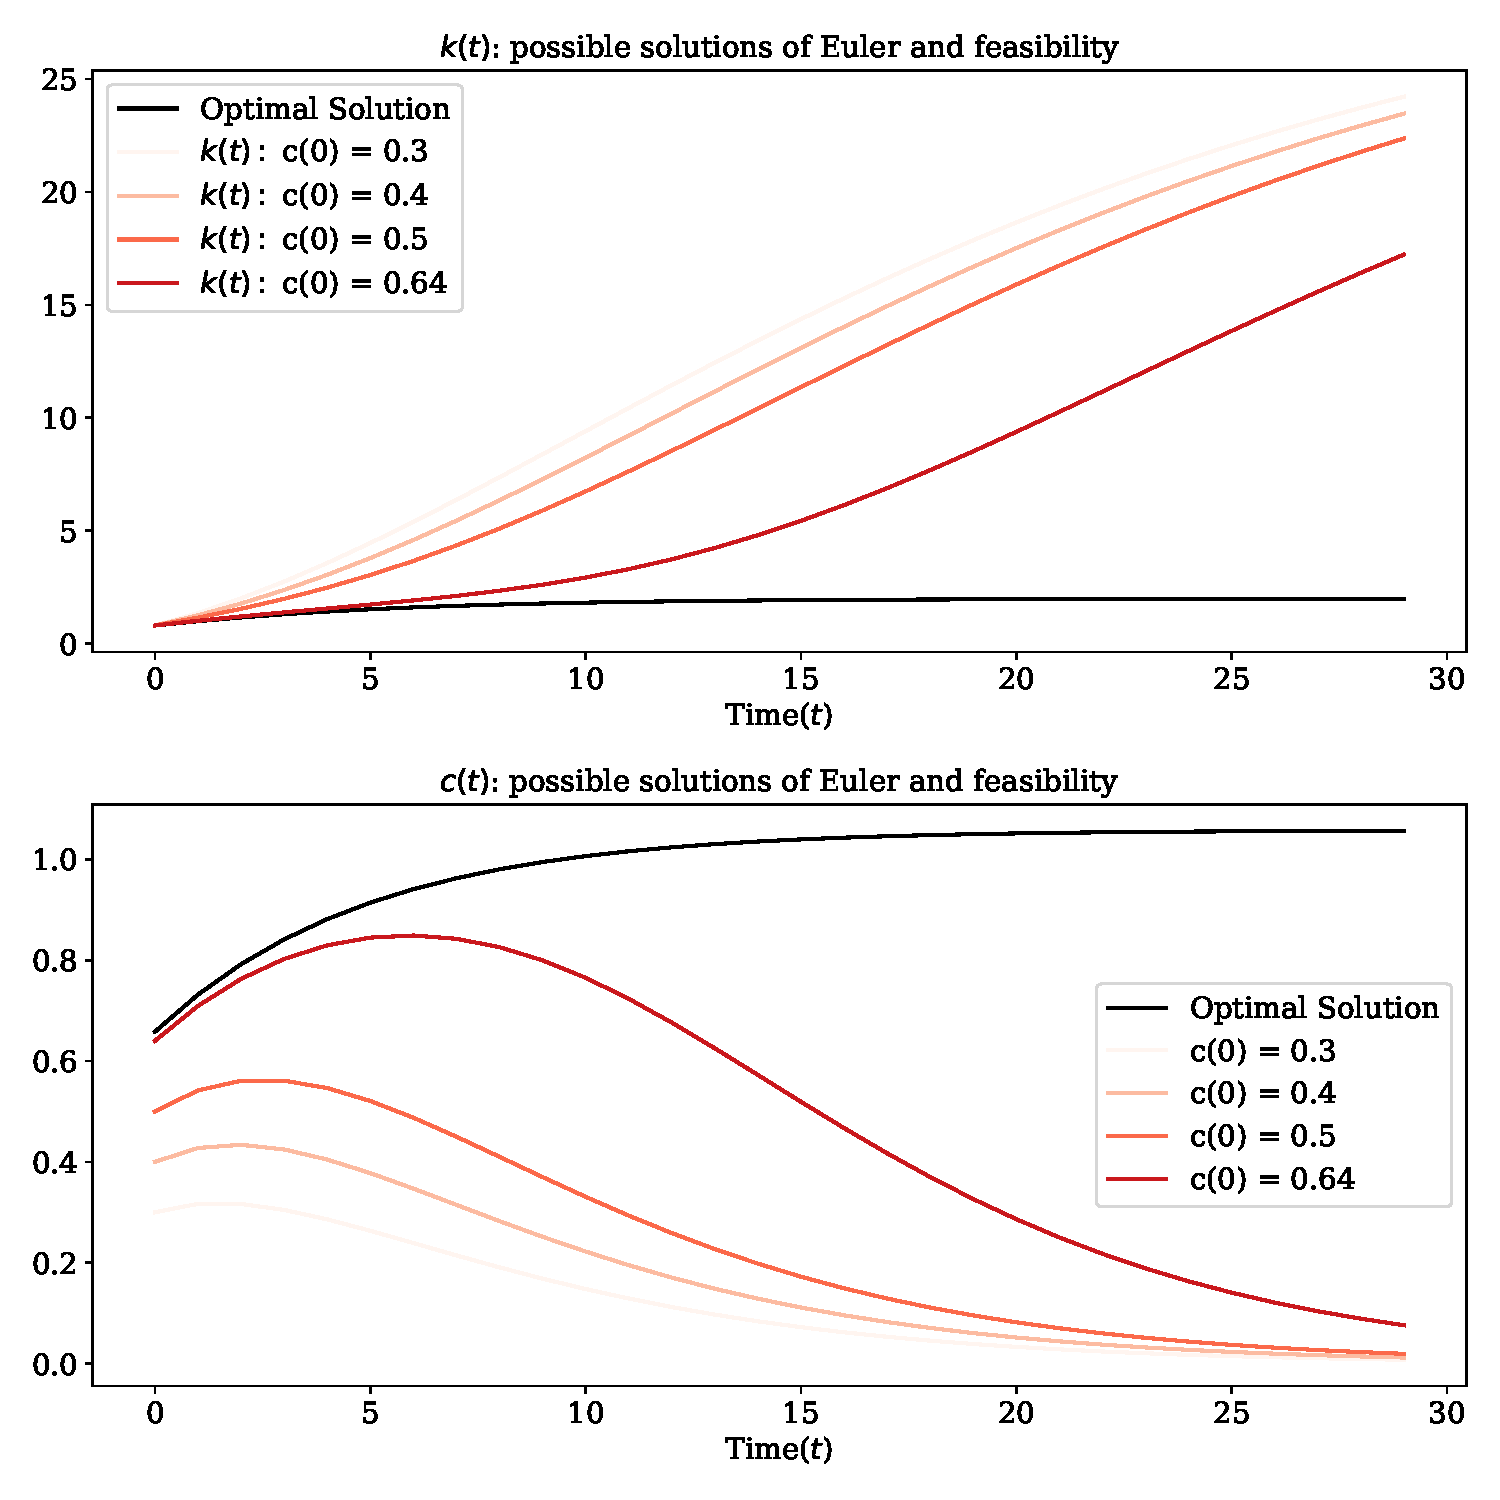
\includegraphics[width=0.65\textwidth]{figs/TVC_violation.pdf}
				\vspace{-7mm}
			\end{figure}
		\end{column}
	\end{columns}
\end{frame}

\begin{frame}{Neoclassical growth model: numerical method}
	\begin{itemize}
		\item Sample for time:  $\mathcal{D} = \{t_1,\cdots,t_N\}$.
		\vspace{0.05in}
		\item TFP process: $z(t+1) = (1+g)z(t)$, given $z(0)$.
		\item A over-parameterized neural network $k_\theta(t)$,
		\vspace{0.05in}
		\item Given $k_\theta(t)$, define the consumption function $c(t;k_{\theta}) = z(t)^{1-\alpha}f(k_{\theta}(t)) +(1-\delta)k_{\theta}(t)-k_{\theta}(t+1)
		$
		\vspace{0.05in}
		 \item \emphcolor{Ignore} the transversality condition and solve
			\hspace*{-5mm}
		\begin{empheq}[box=\tcbhighmath]{align*}
			\hspace*{-4mm}
			\min_{\theta \in \Theta}\Bigg[ \frac{1}{N} \sum_{t \in \mathcal{D}}  \left(\underbrace{\frac{c(t+1;k_{\theta})}{c(t;k_{\theta})} -\beta \big[z(t+1)^{1-\alpha}f'\big(k_{\theta}(t+1)\big)+(1-\delta)\big]}_{\text{Euler residuals}}\right)^2 + \left(\underbrace{k_{\theta}(0)- k_0}_{\text{Initial condition residual}}\right)^2\Bigg]
		\end{empheq}
		\item This minimization should provide an accurate short- and medium-run approximation for the optimal capital and consumption path.
	\end{itemize}
\end{frame}


\begin{frame}{Neoclassical growth model, no TFP growth: results}
	\begin{columns}
		\begin{column}{0.5\textwidth}
			% Content for the left column
			\begin{itemize}
				\item $g=0$, $z(0)=1$.
				\vspace{0.05in}
				\item $\varepsilon_k(t)\equiv \frac{k_\theta(t)-k(t)}{k(t)}$, and  $\varepsilon_c(t)\equiv \frac{c(t;k_\theta)-c(t)}{c(t)}$ 
				\vspace{0.05in}
				\item Benchmark solution: value function iteration.
				\vspace{0.05in}
				\item Results for $100$ different seeds.
				\vspace{0.05in}
				\item Very accurate short- and medium-run approximation.
			\end{itemize}
		\end{column}
		\begin{column}{0.65\textwidth}
			\begin{figure}[t!]
				\centering
				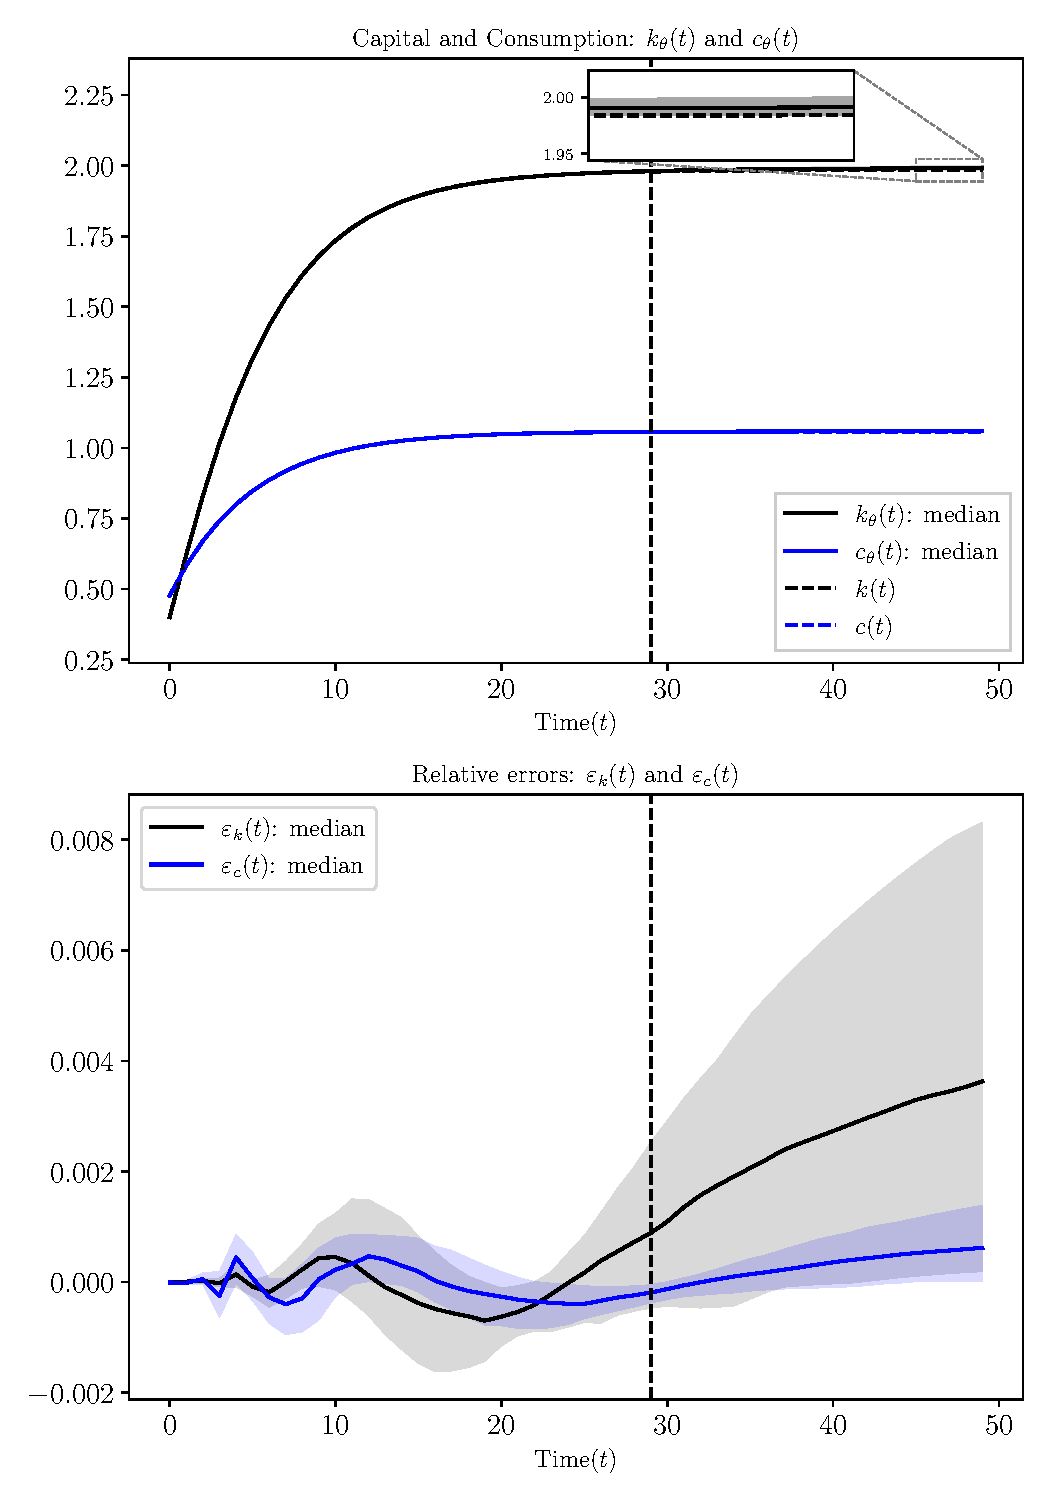
\includegraphics[width=0.5\textwidth]{figs/growth_sequential_g0.pdf}
				\hspace{25mm}
			\end{figure}
		\end{column}
	\end{columns}
\end{frame}

\begin{frame}{Neoclassical growth model with TFP growth: results}
	\begin{columns}
		\begin{column}{0.5\textwidth}
			% Content for the left column
			\begin{itemize}
				\item $g>0$ and $z(0) = 1$.
				\vspace{0.05in}
				\item $k_\theta(t) = e^{\phi t}
				NN_\theta(t)$, $\phi$ is "learnable".
				\vspace{0.05in}
				\item Results for $100$ different seeds.
				\vspace{0.05in}
				\item Very accurate short- and medium-run approximation.
			\end{itemize}
		\end{column}
		\begin{column}{0.5\textwidth}
			\begin{figure}[t!]
				\centering
				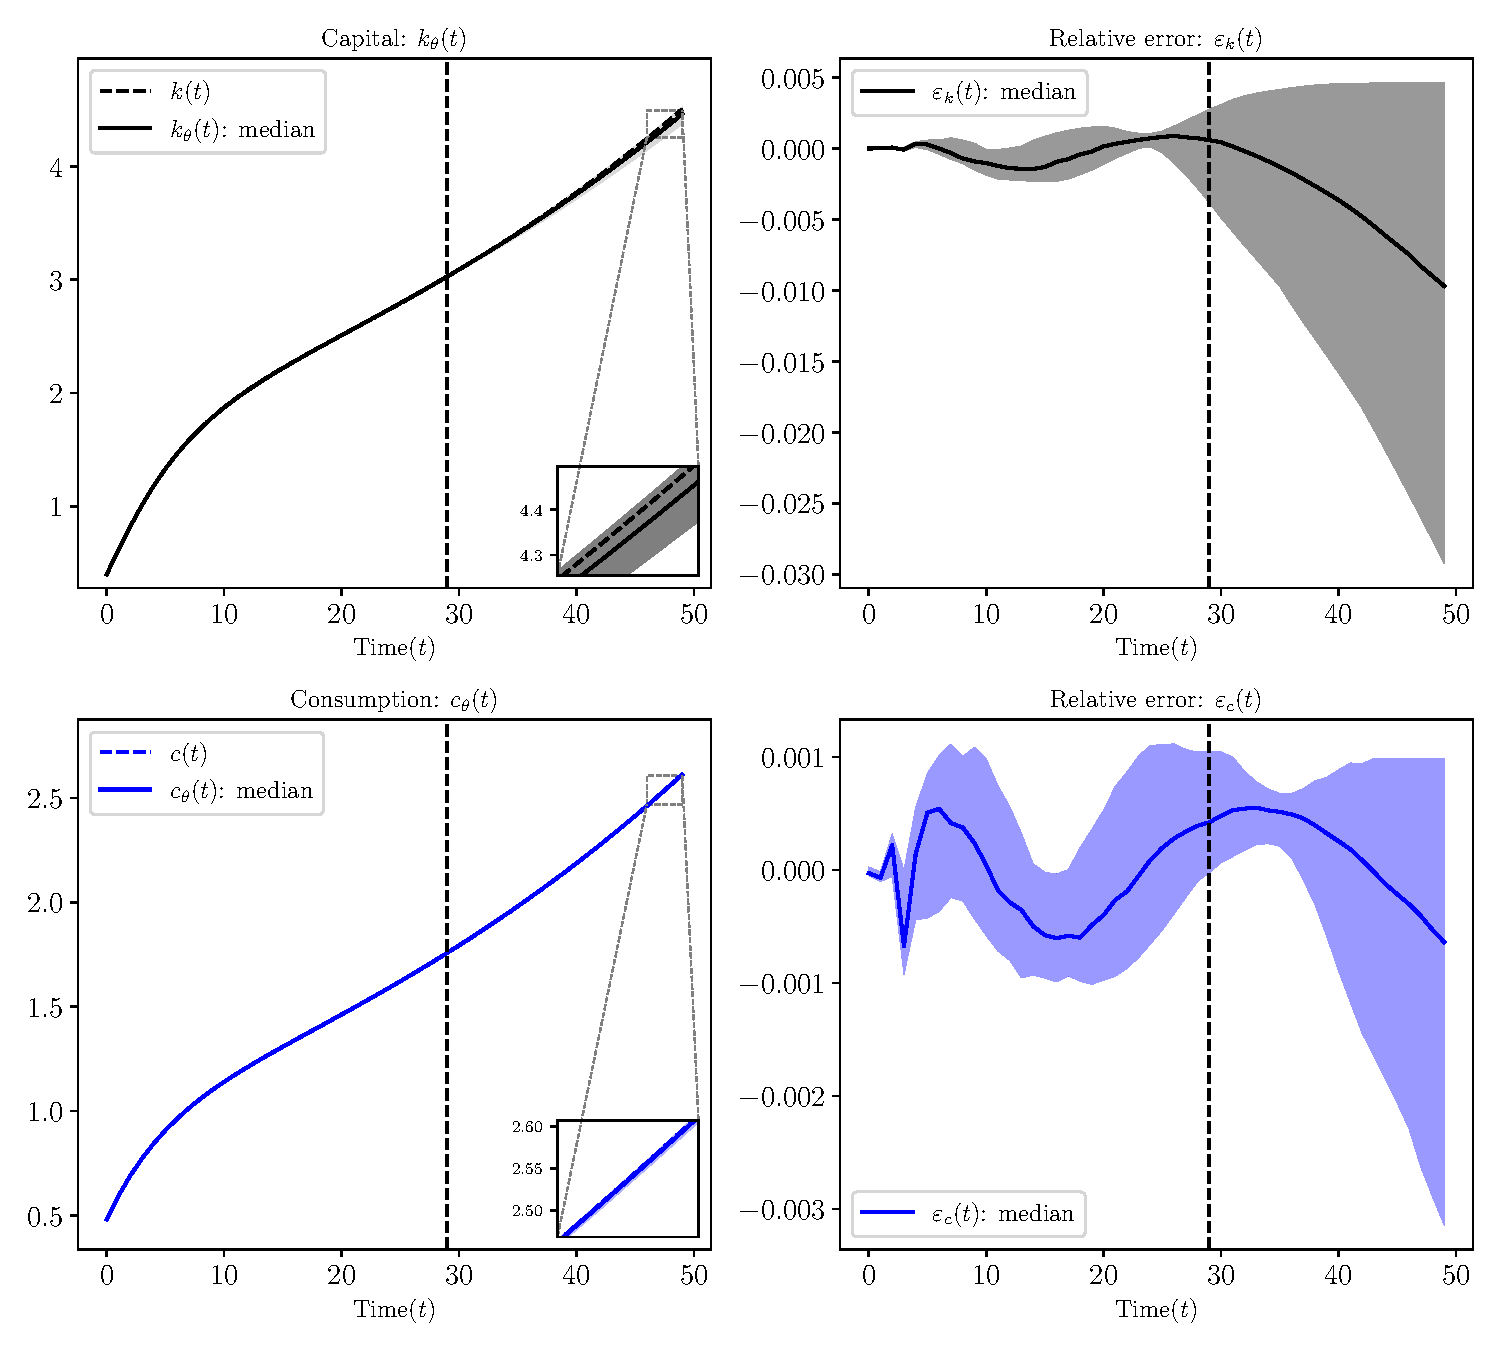
\includegraphics[width=\textwidth]{figs/growth_sequential_g_positive_ensemble.pdf}
				\vspace{-7mm}
			\end{figure}
		\end{column}
	\end{columns}
\end{frame}

\begin{frame}{But, seriously ``in the long run, we are all dead"}

	\begin{columns}
	\begin{column}{0.5\textwidth}
		% Content for the left column
		\begin{itemize}
			\item So far, we have used long time-horizon $\mathcal{D} = \{0,1,\cdots,29\}$.
			\vspace{0.05in}
			\item In other methods, choosing the time-horizon $T$ is a challenge:
			\begin{itemize}
					\item Too large $\rightarrow$ accumulation of errors, and numerical instability. We don't have that problem.
				\item Too small $\rightarrow$ convergence to the steady state too quickly.
			\end{itemize}
			 \vspace{0.05in}
			\item An accurate short-run solution, even for a medium-sized $T$.
		\end{itemize}
	\end{column}
	\begin{column}{0.5\textwidth}
		\begin{figure}[t!]
			\centering
			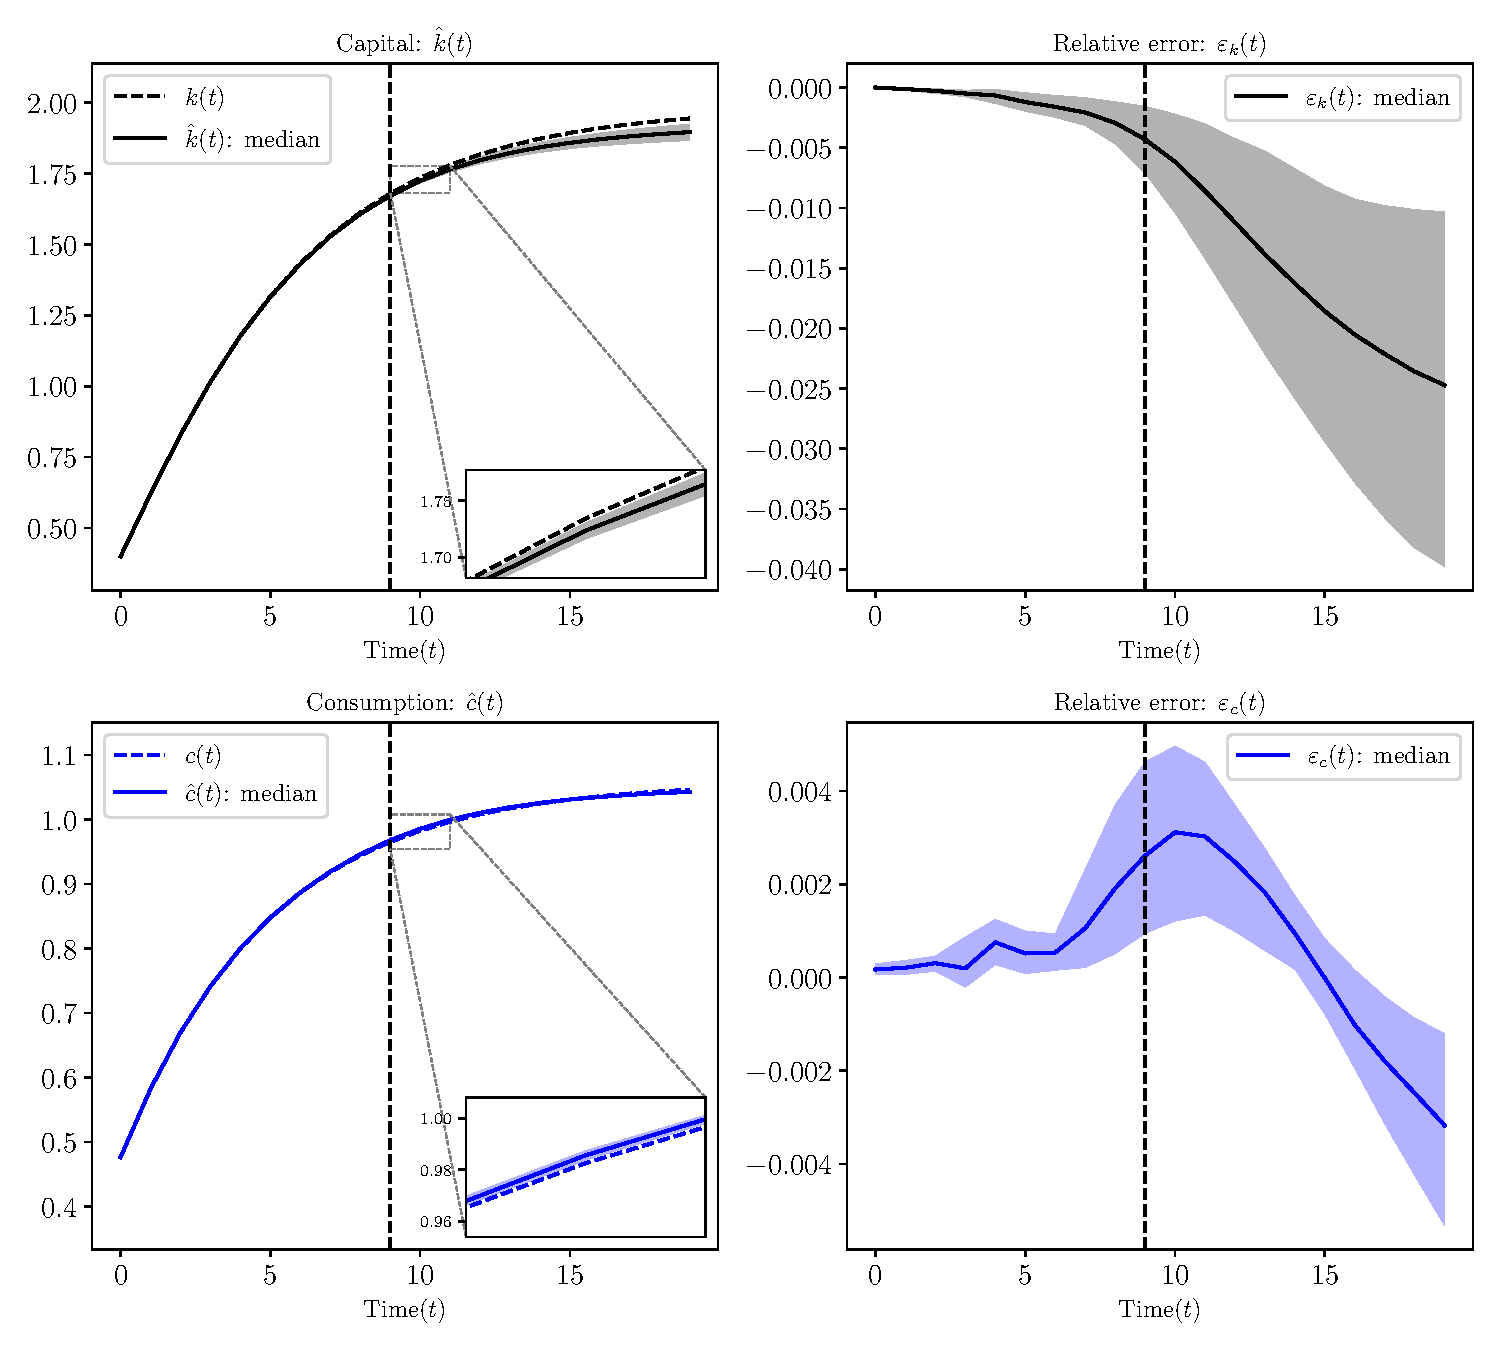
\includegraphics[width=\textwidth]{figs/growth_sequential_g0_t_max_9_ensemble.pdf}
			\vspace{-7mm}
		\end{figure}
	\end{column}
\end{columns}
\end{frame}


\begin{frame}{Do we need a dense and contiguous grid?}

\begin{columns}
	\begin{column}{0.5\textwidth}
		% Content for the left column
		\begin{itemize}
			\item We have used a dense $\mathcal{D} = \{0,1,\cdots,29\}$.
			\vspace{0.05in}
			\item What if 
			\begin{itemize}
				\item $\mathcal{D}(\text{Grid 1}) = \{0, 1, 2, 4, 6, 8, 12, 16, 20, 24, 29\}$
				\item $\mathcal{D}(\text{Grid 2}) = \{0, 1, 4, 8, 12, 18, 24, 29\}$
			\end{itemize}
			\vspace{0.05in}
			\item An accurate short-run solution, even for a sparse grid.
		\end{itemize}
	\end{column}
	\begin{column}{0.5\textwidth}
		\begin{figure}[t!]
			\centering
			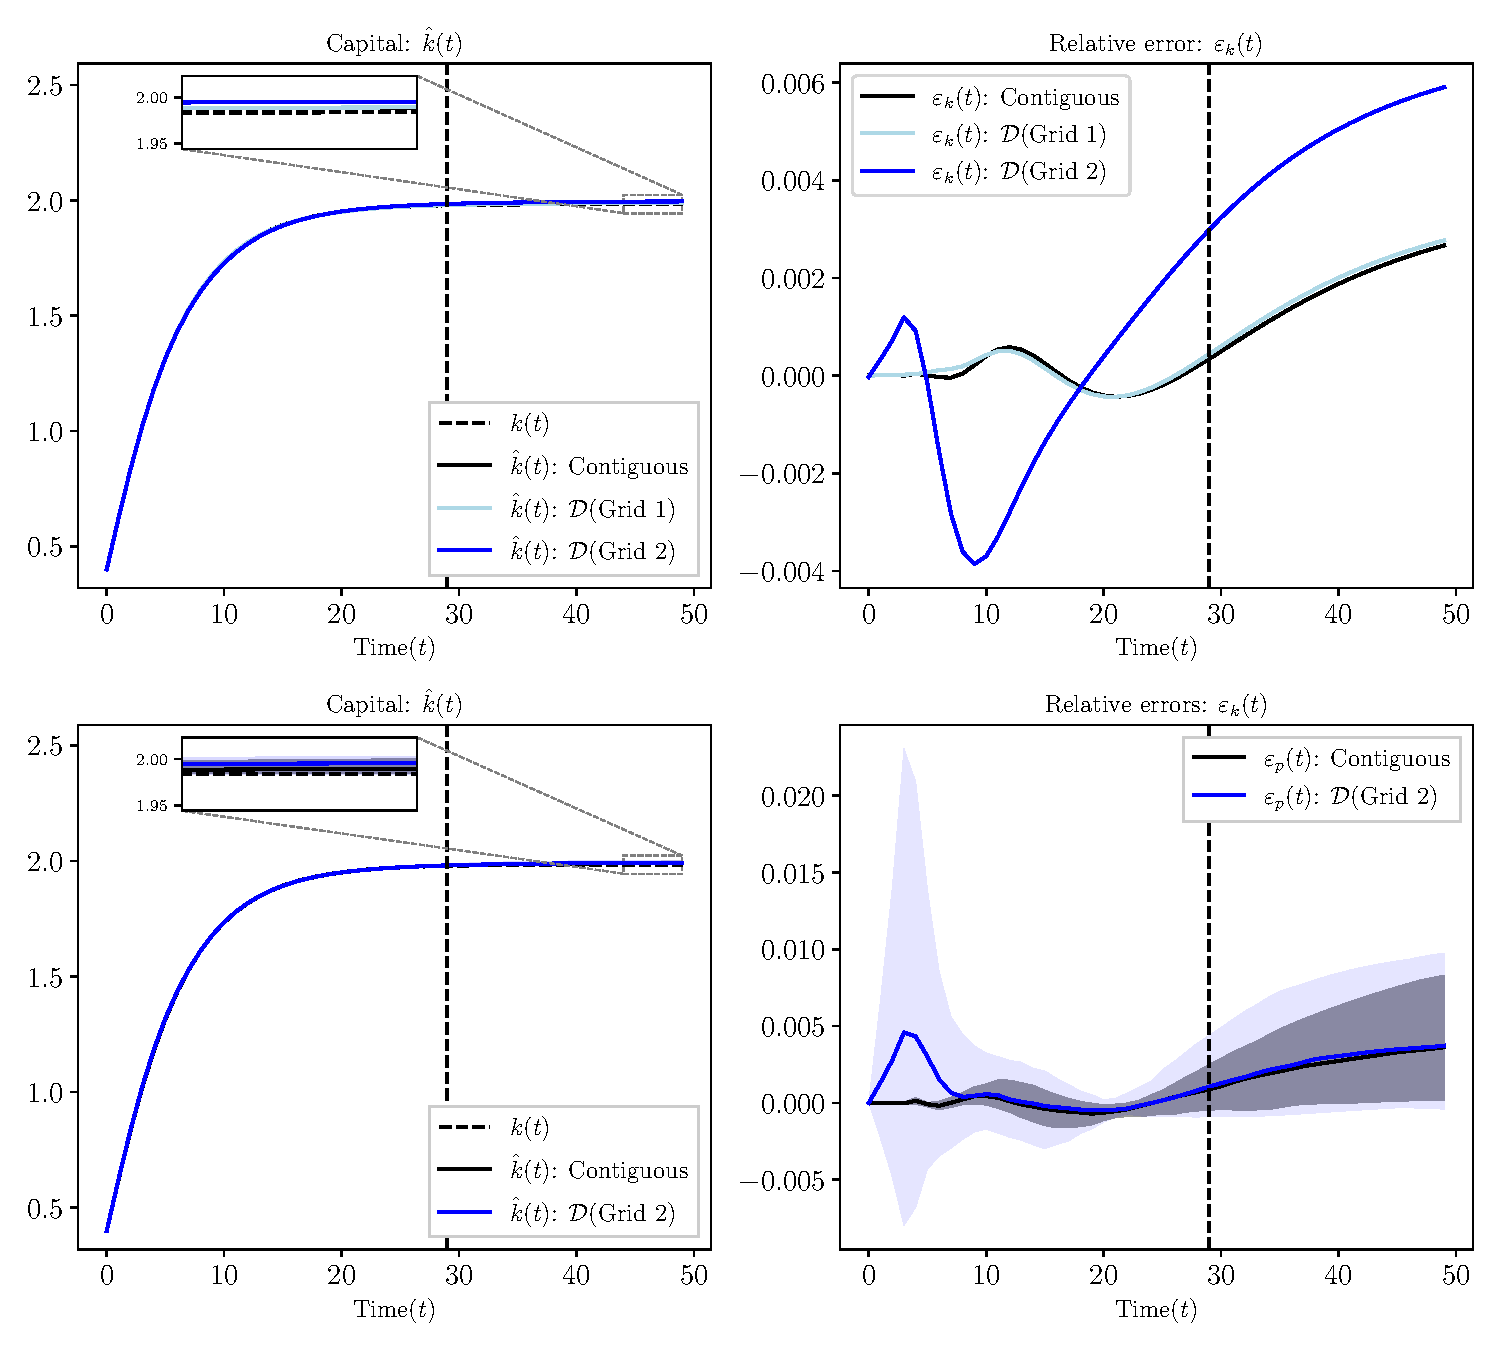
\includegraphics[width=\textwidth]{figs/growth_sequential_g0_grids.pdf}
			\vspace{-7mm}
		\end{figure}
	\end{column}
\end{columns}

\end{frame}


\begin{frame}{Neoclassical growth model: multiple steady-states and hysteresis}
	\begin{itemize}
	\item When there are multiple steady states with saddle-path stability, each with its domain of attraction:
	\vspace{0.05in}
		\begin{itemize}
			\item Can the inductive bias detect there are multiple basins of attraction?
			\item How does the inductive
		bias move us toward the correct steady state for a given initial condition?
		\end{itemize}
	\vspace{0.05in}
	\item Consider a non-concave production function:
	\begin{align*}
		\hspace{-70mm}f(k) \equiv a \max\{k^\alpha, b_1k^\alpha-b_2\}
	\end{align*}
	\item Two steady-states $k_1^*$ and $k_2^*$.
	\vspace{0.05in}
	\item The same numerical procedure.
		\end{itemize}
		
	\vspace{-2cm} % Adjust this spacing as needed
	\hfill
	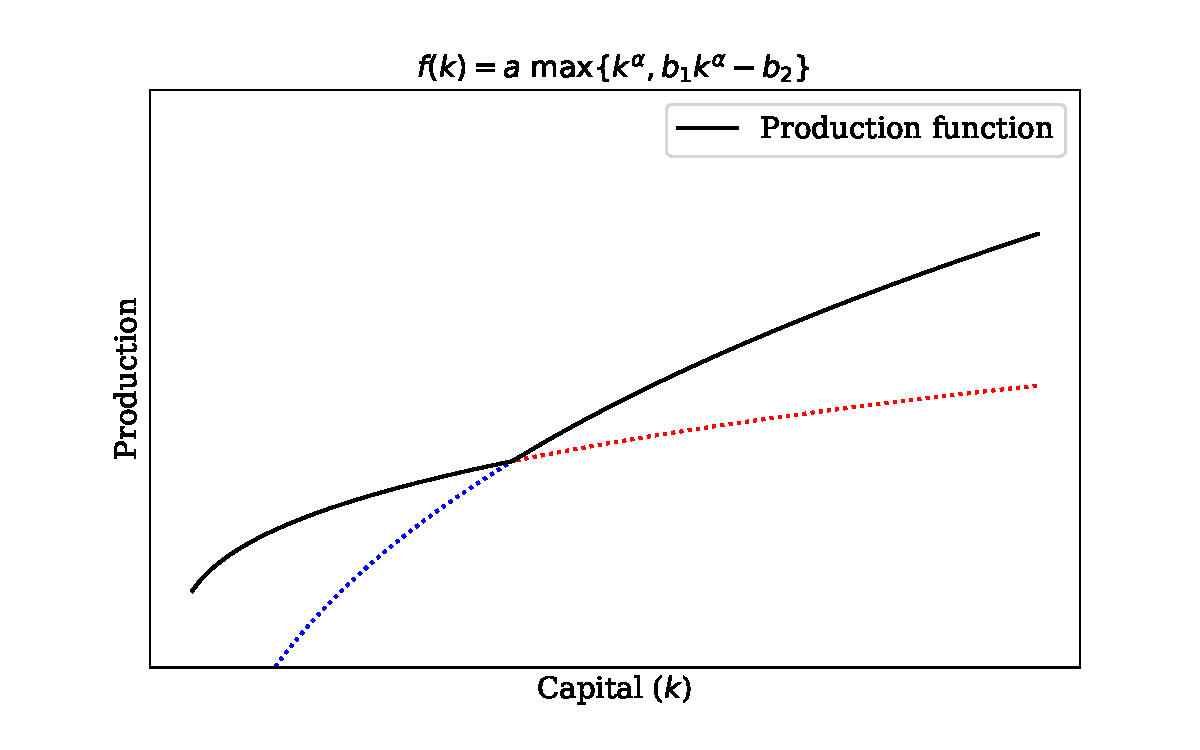
\includegraphics[width=0.55\textwidth]{figs/non_concave_prod_func}
\end{frame}


\begin{frame}{Neoclassical growth model with non-concave production function: results}
	\begin{figure}[t!]
		\centering
		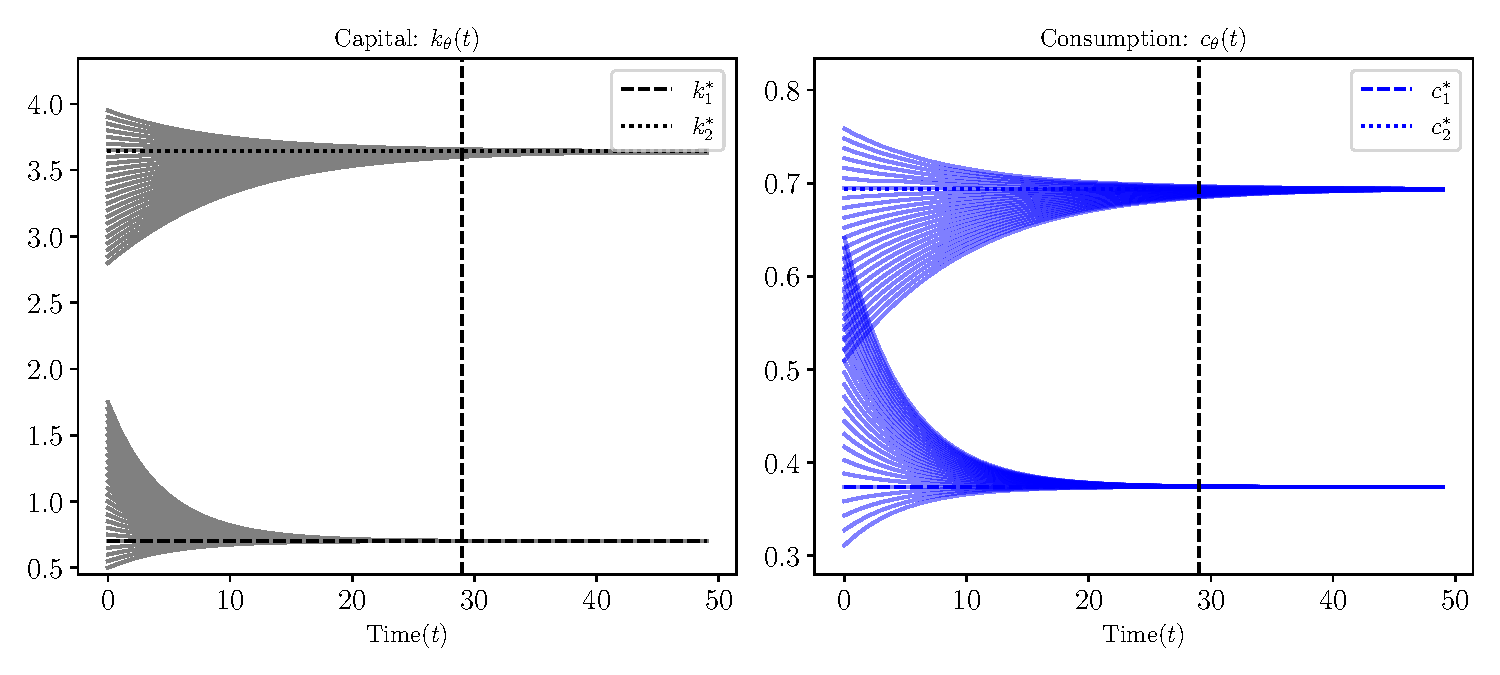
\includegraphics[width=0.75\textwidth]{figs/growth_sequential_multiple_steady_states_var_initial_k_0.pdf}
	\end{figure}
	\begin{itemize}
		\item Different initial conditions in $k_0 \in [0.5,1.75]\cup[2.75,4]$.
		\smallskip
		\item In the vicinity of $k_1^*$ and $k_2^*$ the paths converge to the right steady-states.
	\end{itemize}
\end{frame}

\section{Deep learning is not the only option}

\begin{frame}{Deep learning is not the only option: kernels}
\begin{columns}
	\begin{column}{0.5\textwidth}
		% Content for the left column
			\begin{itemize}
			\item Deep learning might be too ``spooky".
			\smallskip
			\item We can use kernels methods, $K(\cdot,\cdot)$, instead of neural networks and control the RKHS norms.
			\item Focusing on continuous time equivalent of these problems.  
			\item The same results, theoretical guarantees, very fast and robust.
			\item With J Perla, R Childers, and G Pleiss.
		\end{itemize}
	\end{column}
	\begin{column}{0.5\textwidth}
		\begin{figure}[t!]
			\centering
			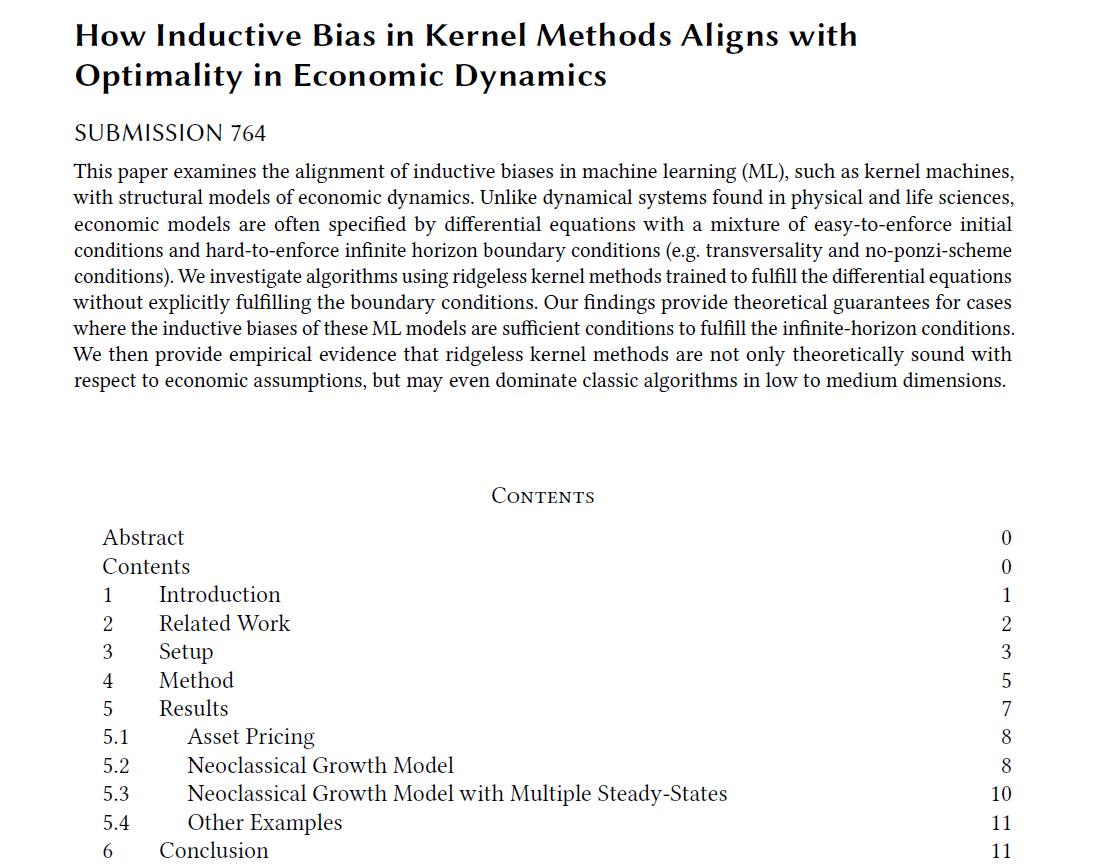
\includegraphics[width=0.9\textwidth]{figs/Kernel}
			\vspace{-7mm}
		\end{figure}
	\end{column}
\end{columns}

\end{frame}

\begin{frame}{Optimal control framework}
	Consider the following problem arising in optimal control:
	
	\begin{align*}
		&\dot{\boldsymbol{x}} = \boldsymbol{F}\left(\boldsymbol{x}(t),\boldsymbol{y}(t)\right)\\
		&\dot{\boldsymbol{\mu}} = r\boldsymbol{\mu}(t)-\boldsymbol{\mu}(t)\odot \boldsymbol{G}\left(\boldsymbol{x}(t),\boldsymbol{\mu}(t),\boldsymbol{y}(t)\right)\\
		&\boldsymbol{0}= \boldsymbol{H}\left(\boldsymbol{x}(t),\boldsymbol{\mu}(t),\boldsymbol{y}(t)\right)\\
		&\boldsymbol{x}(0) = \boldsymbol{x}_0
	\end{align*}
	\begin{itemize}
		\item \emph{State variables} $\boldsymbol{x}(t)\in\R^{M}$, initial condition $\boldsymbol{x}_0$; \emph{co-state variables} $\boldsymbol{\mu}(t)\in\R^{M}$; \emph{jump variables} $\boldsymbol{y}(t)\in\R^{P}$
		\item This problem is \emphcolor{ill-posed} and can have infinitely many solutions.
	\end{itemize}
\end{frame}

\begin{frame}{Transversality condition: an asymptotic boundary condition}
	\begin{align*}
		\lim_{t\rightarrow \infty} e^{-rt} \boldsymbol{x}(t)\odot\boldsymbol{\mu}(t) = \boldsymbol{0}
	\end{align*}
	\begin{itemize}
	\item The transversality condition is an asymptotic boundary condition.
	\item We typically assume a finite time horizon \( T \) and shoot for the \emph{finite} steady state \( \boldsymbol{x}^* \), \( \boldsymbol{\mu}^* \), and \( \boldsymbol{y}^* \).
	\item This approach is straightforward in low dimensions but becomes significantly more challenging in high-dimensional settings.
	\end{itemize}
\end{frame}

\begin{frame}{Optimal control framework: an example, Ramsey–Cass–Koopmans model}
\begin{itemize}
	\item Classic Ramsey–Cass–Koopmans
	\begin{align*}
		\dot{k}(t) &= f\left(k(t)\right) - c(t) - \delta k(t)\\
		\dot{\mu}(t) &= r \mu(t) - \mu(t) \left[f'(k(t)) - \delta \right] \\
		0 &= c(t)\mu(t) - 1\\
		k(0)& = k_0\\
		0 &= \lim_{t\rightarrow \infty} e^{-r t}k(t)\mu(t)
	\end{align*}
\item $f(\cdot)$ is the production function, $r$ discount rate, and $\delta$ is the depreciation.
\end{itemize}
\end{frame}

\begin{frame}{What does the violation of the transversality condition look like?}
	\begin{columns}
		\begin{column}{0.5\textwidth}
			% Content for the left column
			\begin{itemize}
				\item All paths solve the ordinarily differential equations ans the algebraic equation.
				\vspace{0.05in}
				\item The solutions that violate the transversality condition $\lim_{t\rightarrow \infty}{\dot{\mu}} = \infty $ and $\lim_{t\rightarrow \infty}{\mu} = \infty $
				\begin{itemize}
					\item Diverges faster than $e^{rt}$.
				\end{itemize}
			\end{itemize}
		\end{column}
		\begin{column}{0.5\textwidth}
			\begin{figure}[t!]
				\centering
				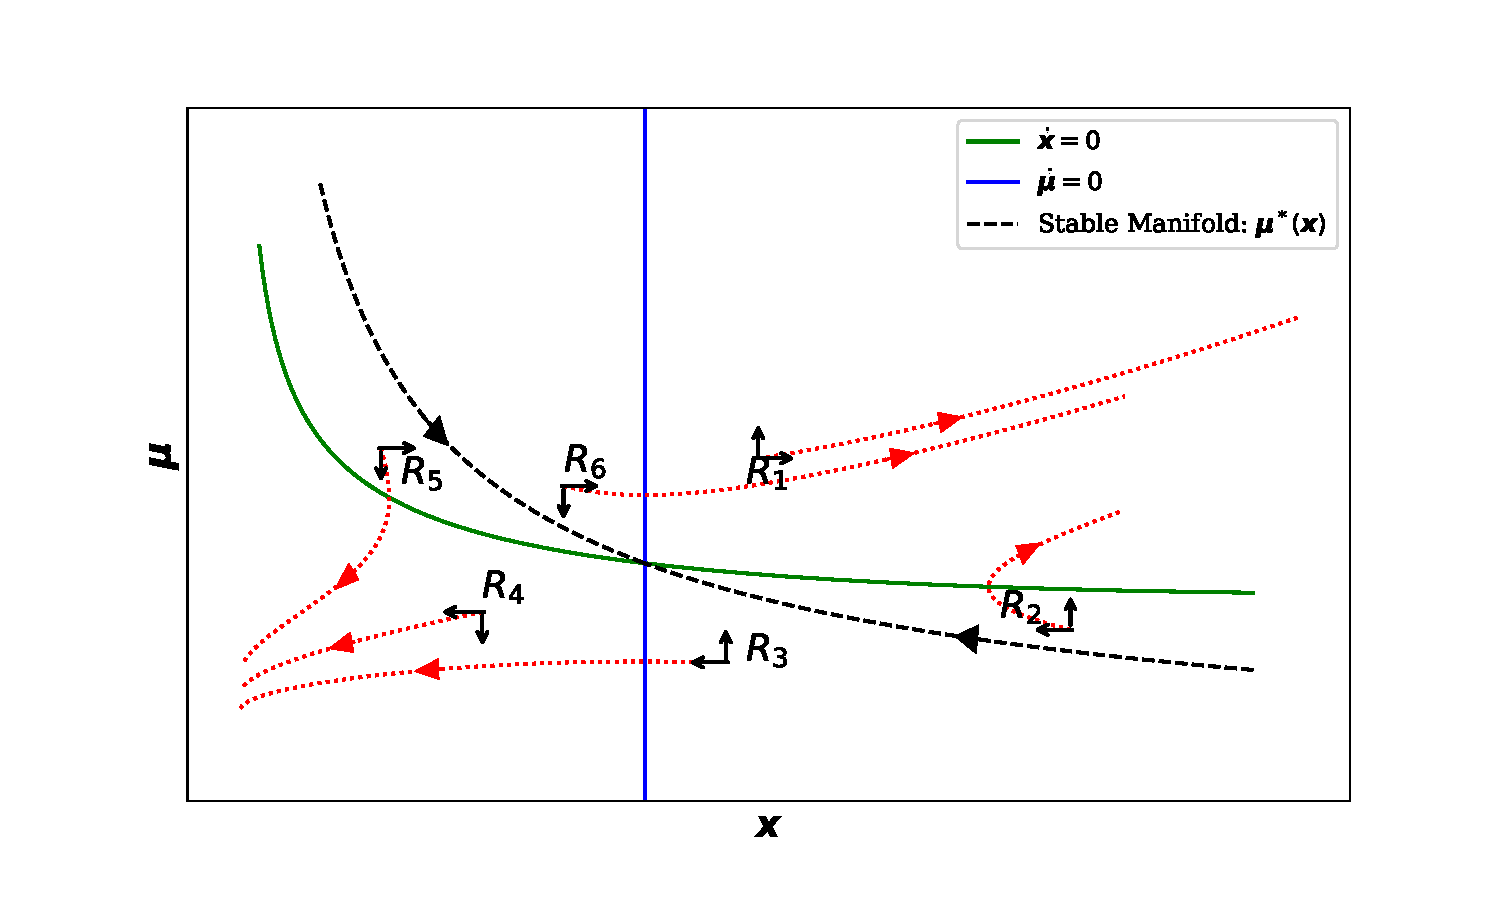
\includegraphics[width=\textwidth]{figs/phase_diagram_mu_k.pdf}
				\vspace{-7mm}
			\end{figure}
		\end{column}
	\end{columns}
\end{frame}

\begin{frame}{Kernel approximation}
Approximating the derivatives with a kernel:
	\begin{align*}
		\hat{\boldsymbol{x}}(t) = \boldsymbol{x}_0 + \int_0^t \hat{\dot{\boldsymbol{x}}}(\tau) d\tau, \qquad
		\hat{\boldsymbol{\mu}}(t) = \hat{\boldsymbol{\mu}}_0 + \int_0^t \hat{\dot{\boldsymbol{\mu}}}(\tau) d\tau, \qquad
		\hat{\boldsymbol{y}}(t) = \hat{\boldsymbol{y}}_0 + \int_0^t \hat{\dot{\boldsymbol{y}}}(\tau) d\tau,\\
		\hat{\dot{\boldsymbol{x}}}(t)  = \sum_{j=1}^N \boldsymbol{\alpha}^x_j K(t, t_j), \qquad
		\hat{\dot{\boldsymbol{\mu}}}(t)  = \sum_{j=1}^N \boldsymbol{\alpha}^\mu_j K(t, t_j), \qquad
		\hat{\dot{\boldsymbol{y}}}(t)  = \sum_{j=1}^N \boldsymbol{\alpha}^y_j K(t, t_j)
	\end{align*}
\begin{itemize}
	\item $\boldsymbol{x}_0$ is given.
	\item $\hat{\boldsymbol{\mu}}_0$, $\hat{\boldsymbol{y}}_0$, $\boldsymbol{\alpha}^x$,
	$\boldsymbol{\alpha}^\mu$, and $\boldsymbol{\alpha}^y$ are learnable parameters.
	\item $K(\cdot,\cdot)$ is the kernel.
\end{itemize}
\end{frame}

\begin{frame}{Approximate solution: Algorithm}
	\begin{align*}
		\min_{\substack{
			\hat{\boldsymbol{x}}(t)	\in \mathcal{H}^{M}, \hat{\boldsymbol{\mu}}(t) \in \mathcal{H}^{M}, \\\hat{\boldsymbol{y}}(t) \in \mathcal{H}^{P} 
		}}\, & \left(
	\sum_{m=1}^{M}\,  \Vert \hat{\dot{x}}^{(m)}  \Vert^2_{\mathcal{H}}  + \sum_{m=1}^{M}\, \Vert \hat{\dot{\mu}}^{(m)}  \Vert^2_{\mathcal{H}}  \right) \\
	\text{s.t.}\, &\hat{\dot{\boldsymbol{x}}} = \boldsymbol{F}\left(\hat{\boldsymbol{x}}(t),\hat{\boldsymbol{y}}(t)\right)\\
	&\hat{\dot{\boldsymbol{\mu}}} = r\hat{\boldsymbol{\mu}}(t)-\hat{\boldsymbol{\mu}}(t)\odot \boldsymbol{G}\left(\hat{\boldsymbol{x}}(t),\hat{\boldsymbol{\mu}}(t),\hat{\boldsymbol{y}}(t)\right)\\
	&\boldsymbol{0}= \boldsymbol{H}\left(\hat{\boldsymbol{x}}(t),\hat{\boldsymbol{\mu}}(t),\hat{\boldsymbol{y}}(t)\right)
	\end{align*}

\begin{itemize}
	\item The objective function penalizes explosive paths.
	\item Constraints solve the "first order conditions".
\end{itemize}	
	
\end{frame}


\begin{frame}{Application: Growth with human and physical capital, a mid-size problem}

\begin{align*}
	\dot{k}(t)  = i_{k}(t)-\delta_k k(t), &\qquad \dot{h}(t)  = i_{h}(t)-\delta_h h(t),\\
	\dot{\mu}_k(t) = r\mu_k(t)- \mu_k(t) \left[ f_k\left(k(t),h(t)\right) -\delta_k \right], & \qquad 	\dot{\mu}_h(t) = r\mu_h(t)- \mu_h(t) \left[ f_h\left(k(t),h(t)\right) -\delta_h \right]\\
	0  = \mu_{k}(t)c(t) -1, &\qquad 0  = \mu_{k}(t)-\mu_h(t)\\
	0  =   f\left(k(t),h(t)\right) - c(t) -  i_{k}(t) -  i_{h}(t)&, 
\end{align*}
for given initial conditions $k(0) = k_0$, $h(0) = h_0 $, and two transversality conditions 
\begin{align*}
	0 & = \lim_{t\rightarrow \infty} e^{-r t}k(t)\mu_k(t), &\qquad 	0 & = \lim_{t\rightarrow \infty} e^{-r t}h(t)\mu_h(t).
\end{align*}
\begin{itemize}
	\item $\boldsymbol{x}(t) = \left[k(t),h(t)\right]^T$, $\boldsymbol{\mu}(t) = \left[\mu_k(t),\mu_h(t)\right]^T$, $\boldsymbol{y}(t) = \left[i_k(t),i_h(t),c(t)\right]^T$ 
\end{itemize}
\end{frame}

\begin{frame}{Results}
			\begin{columns}
			\begin{column}{0.5\textwidth}
				% Content for the left column
				\begin{itemize}
					\item Accurate short- and medium-run solution.
					\vspace{0.05in}
					\item The solution ``learns" the steady state.
				\end{itemize}
			\end{column}
			\begin{column}{0.42\textwidth}
				\begin{figure}[t!]
					\centering
					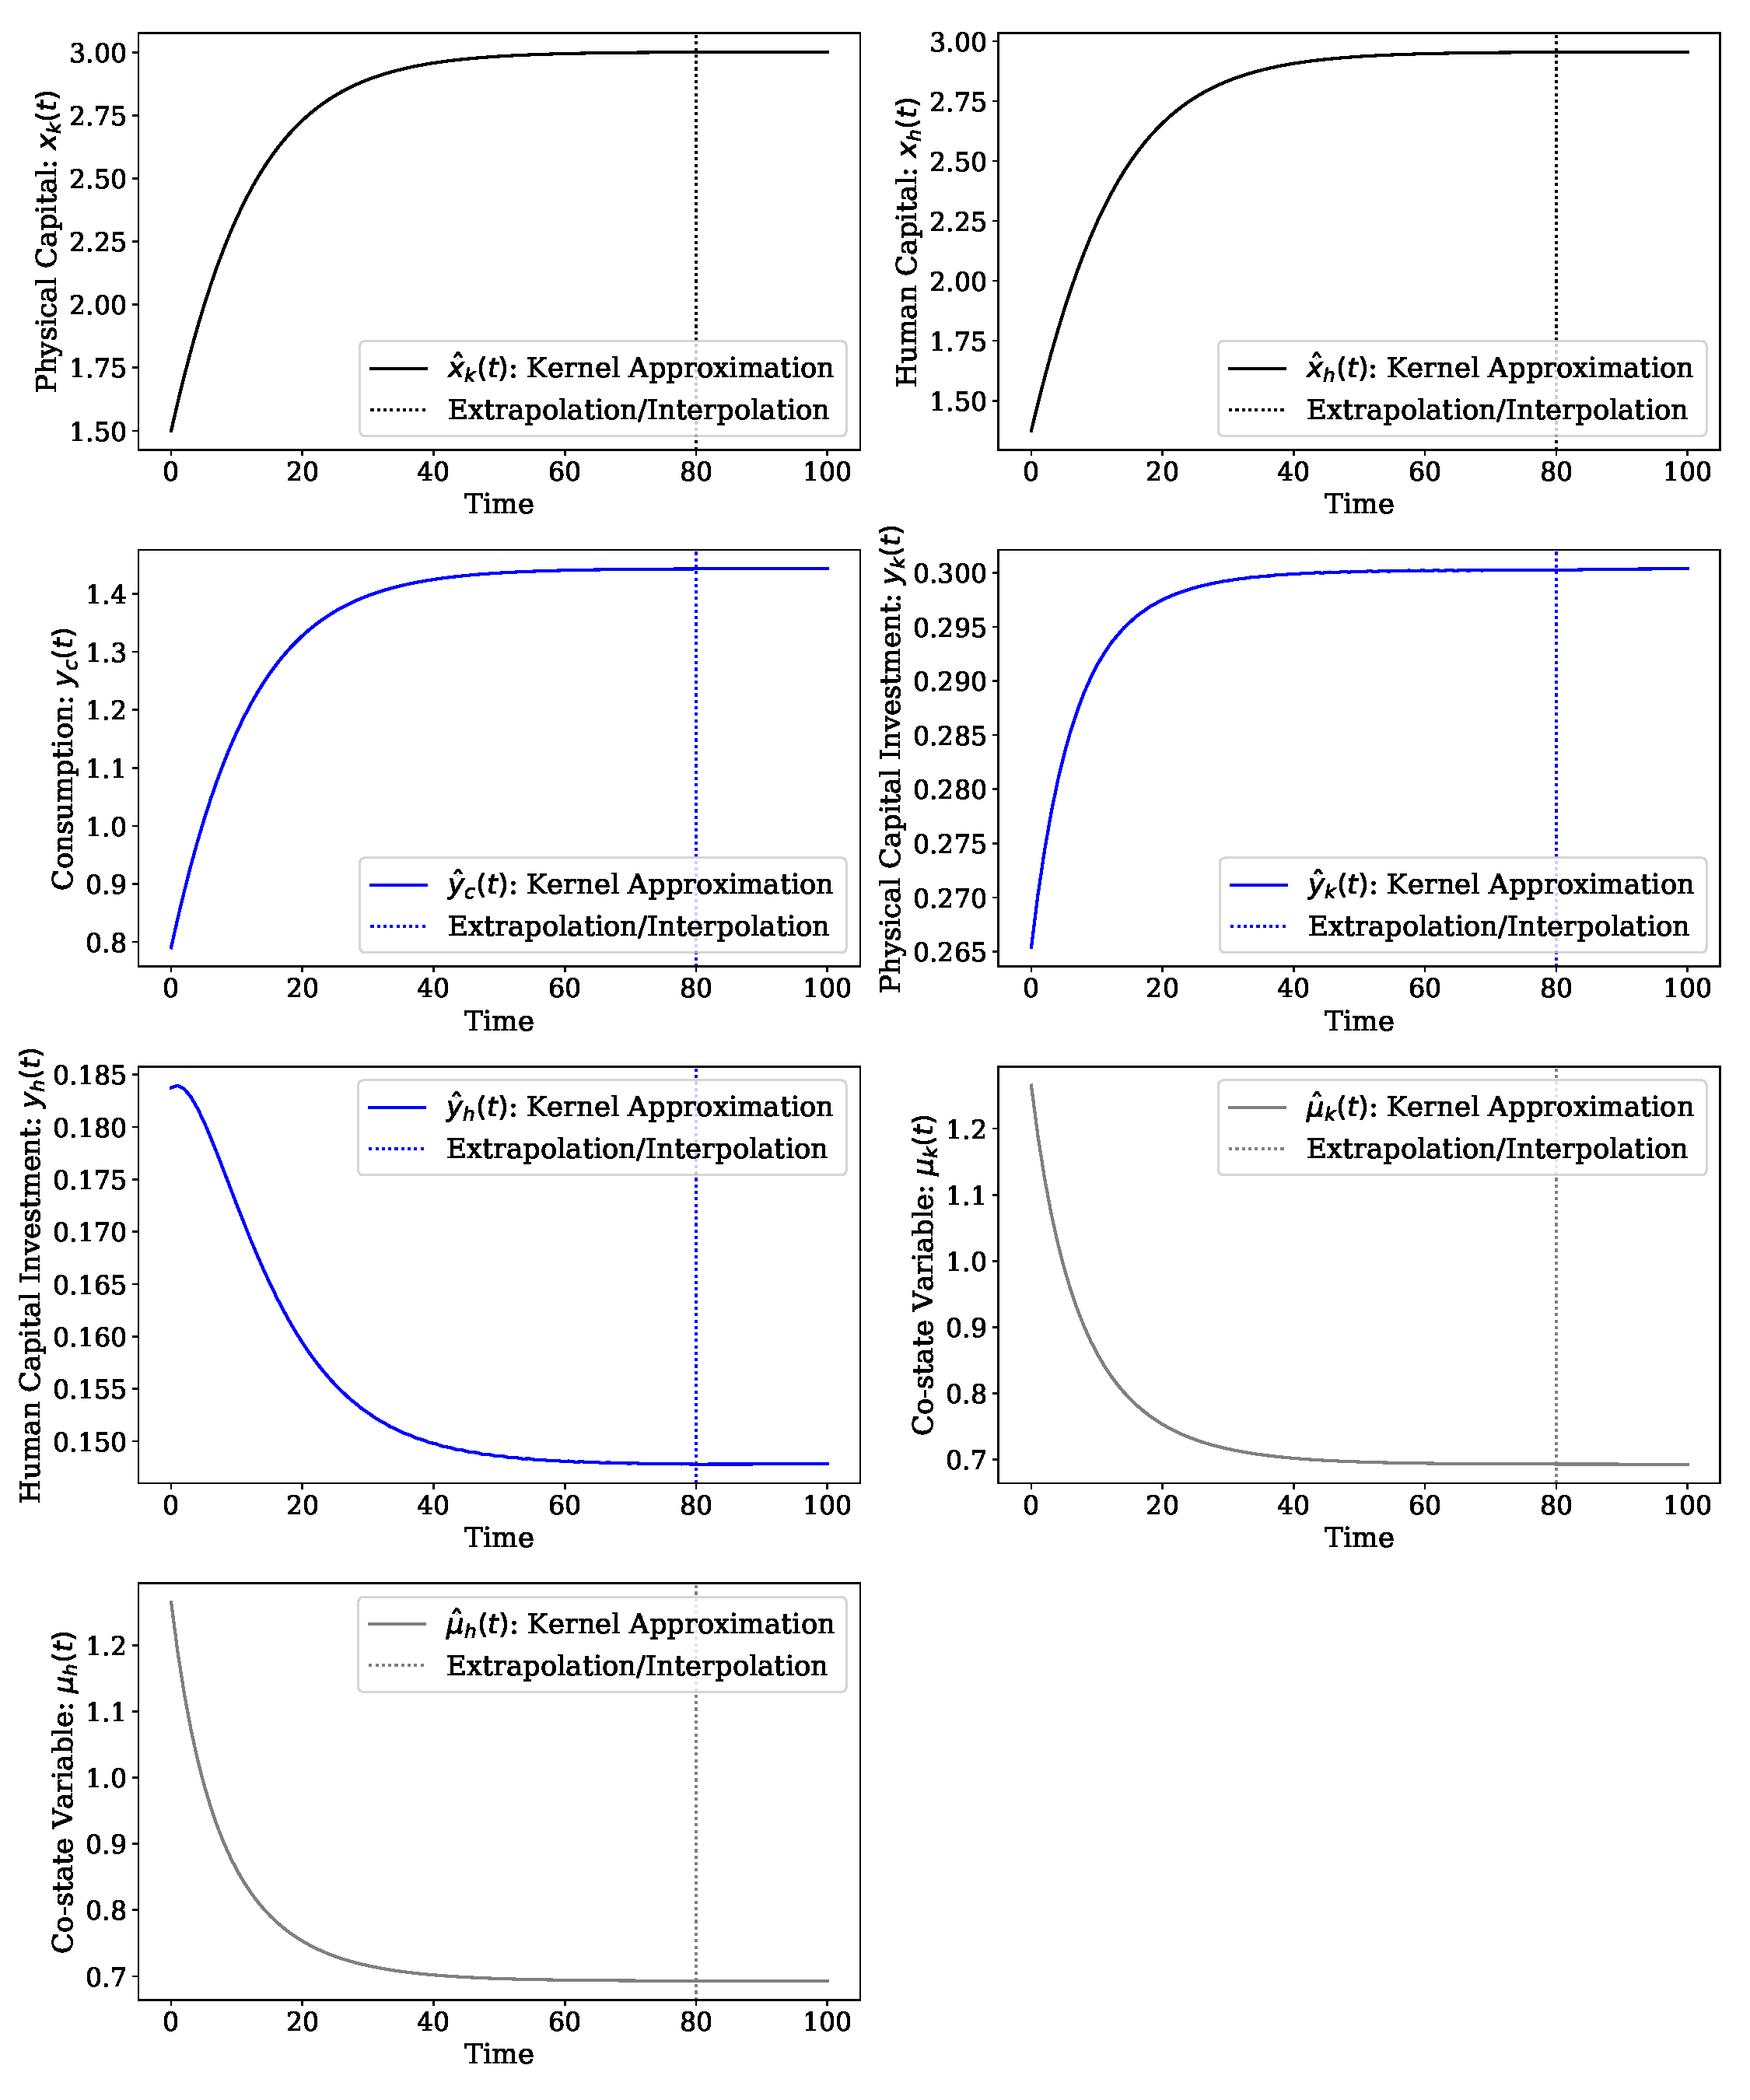
\includegraphics[width=\textwidth]{figs/neoclassical_human_capital.pdf}
					\vspace{-7mm}
				\end{figure}
			\end{column}
		\end{columns}
\end{frame}

\section{\textcolor{PennBlue}{Back to deep learning: Recursive neoclassical growth model and the transversality condition }}

\begin{frame}{Recursive formulation (with a possible BGP)}
	
	Skipping the Bellman formulation and going to the first order conditions in the state space , i.e., $(k,z)$
	\begin{align*}
		\quad & u'(c(k,z)) = \beta  u'(c(k'(k,z),z'))\big[z'^{1-\alpha}f'(k'(k,z))+ 1 -\delta\big]                                          \\
		\quad & k'(k,z) = z^{1-\alpha}f(k) + (1-\delta)k - c(k,z)                                                                          \\
		\quad & z' = (1+g)z                                                                                                                \\
		& k'\geq0                                                                                       \\
		\quad & 0 = \lim_{T\rightarrow \infty} \beta^T  u'(c_T)k_{T+1}\label{eq:transversality-req-rbc-sequential} \quad \forall (k_0,z_0)\in \Xdom
	\end{align*}
	\begin{itemize}
		\item Preferences: $u(c) = \frac{c^{1-\sigma}-1}{1-\sigma}$, $\sigma > 0$, $\lim_{c\rightarrow 0} u'(c) = \infty$, and $\beta \in (0,1)$.			\smallskip
		\item Cobb-Douglas production function: $f(k) = k^{\alpha}$, $\alpha \in (0,1)$ before scaling by TFP $z$.
	\end{itemize}
\end{frame}

\begin{frame}{Interpolation problem: the optimization problem}
	\begin{itemize}
		\item A set of points $\mathcal{D} = \{k_1,\ldots,k_{N_k}\}\times \{z_1,\ldots,z_{N_z}\}$.
		\item A family of over-parameterized  functions $k'(\cdot,\cdot;\theta) \in \mathcal{H}(\Theta)$.
		\item Use the feasibility condition and define $c(k,z;k') \equiv z^{1-\alpha} f(k)+(1-\delta)k-k'(k,z)$.
	\end{itemize}
	
	
	In practice we minimize the Euler residuals: 
	\begin{empheq}[box=\tcbhighmath]{align*}
		\min_{\theta \in \Theta} \frac{1}{|\mathcal{D}|}\sum_{(k,z) \in \mathcal{D}} \left[\underbrace{ \frac{u'\bigg(c\big(k,z;k'(.;\theta)\big)\bigg)}{u'\bigg(c\big(k'(k,z;\theta),(1+g)z;k'(.;\theta)\big)\bigg)} -  \beta 
			\left[\left((1+g)z\right)^{1-\alpha} f'\left(k'(k,z;\theta)\right) + 1-\delta\right]}_{\text{Euler residual}} \right]^2
	\end{empheq}
\end{frame}


\begin{frame}{Interpolation problem: without the transversality condition}
	\begin{itemize}
		\item This minimization \emphcolor{does not contain} the transversality condition.
		\smallskip
		\begin{itemize}
			\item Without the transversality condition it has more than one minima.
		\end{itemize}
		\bigskip
		\item \emphcolor{No explicit} norm regularization.
		\bigskip
		\item Does the implicit bias weed out the solutions that violate the transversality condition? 
		\bigskip
		Let's analyze this more rigorously.
	\end{itemize}
\end{frame}


\begin{frame}{Is the transversality condition necessary? Case of g = 0, z = 1}
	\begin{figure}[htb]
		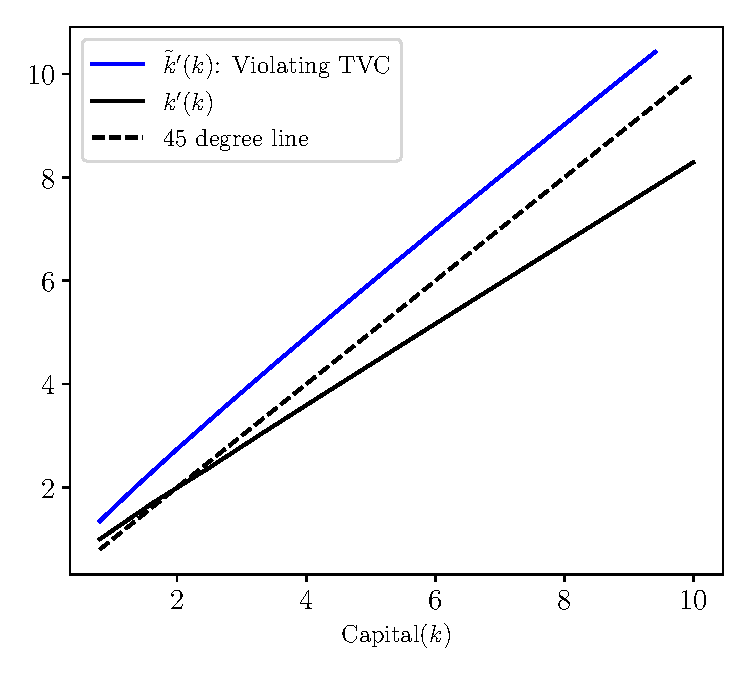
\includegraphics[width=8cm]{figs/growth_recursive_analytic_solutions.pdf}
	\end{figure}
	\begin{itemize}
		\item The solutions that violate the transversality condition are above the one that do not.
		\item They have bigger derivatives. Therefore, they have bigger norms:
		\begin{align}
			0\leq \|k'\|_S < \|\tilde{k}'\|_S.
		\end{align}
	\end{itemize}
\end{frame}

\begin{frame}[label = res-rec]
	\frametitle{Results: one initial condition}
	\begin{minipage}[t]{0.4\textwidth}
		\raisebox{-\height+0.7\baselineskip}{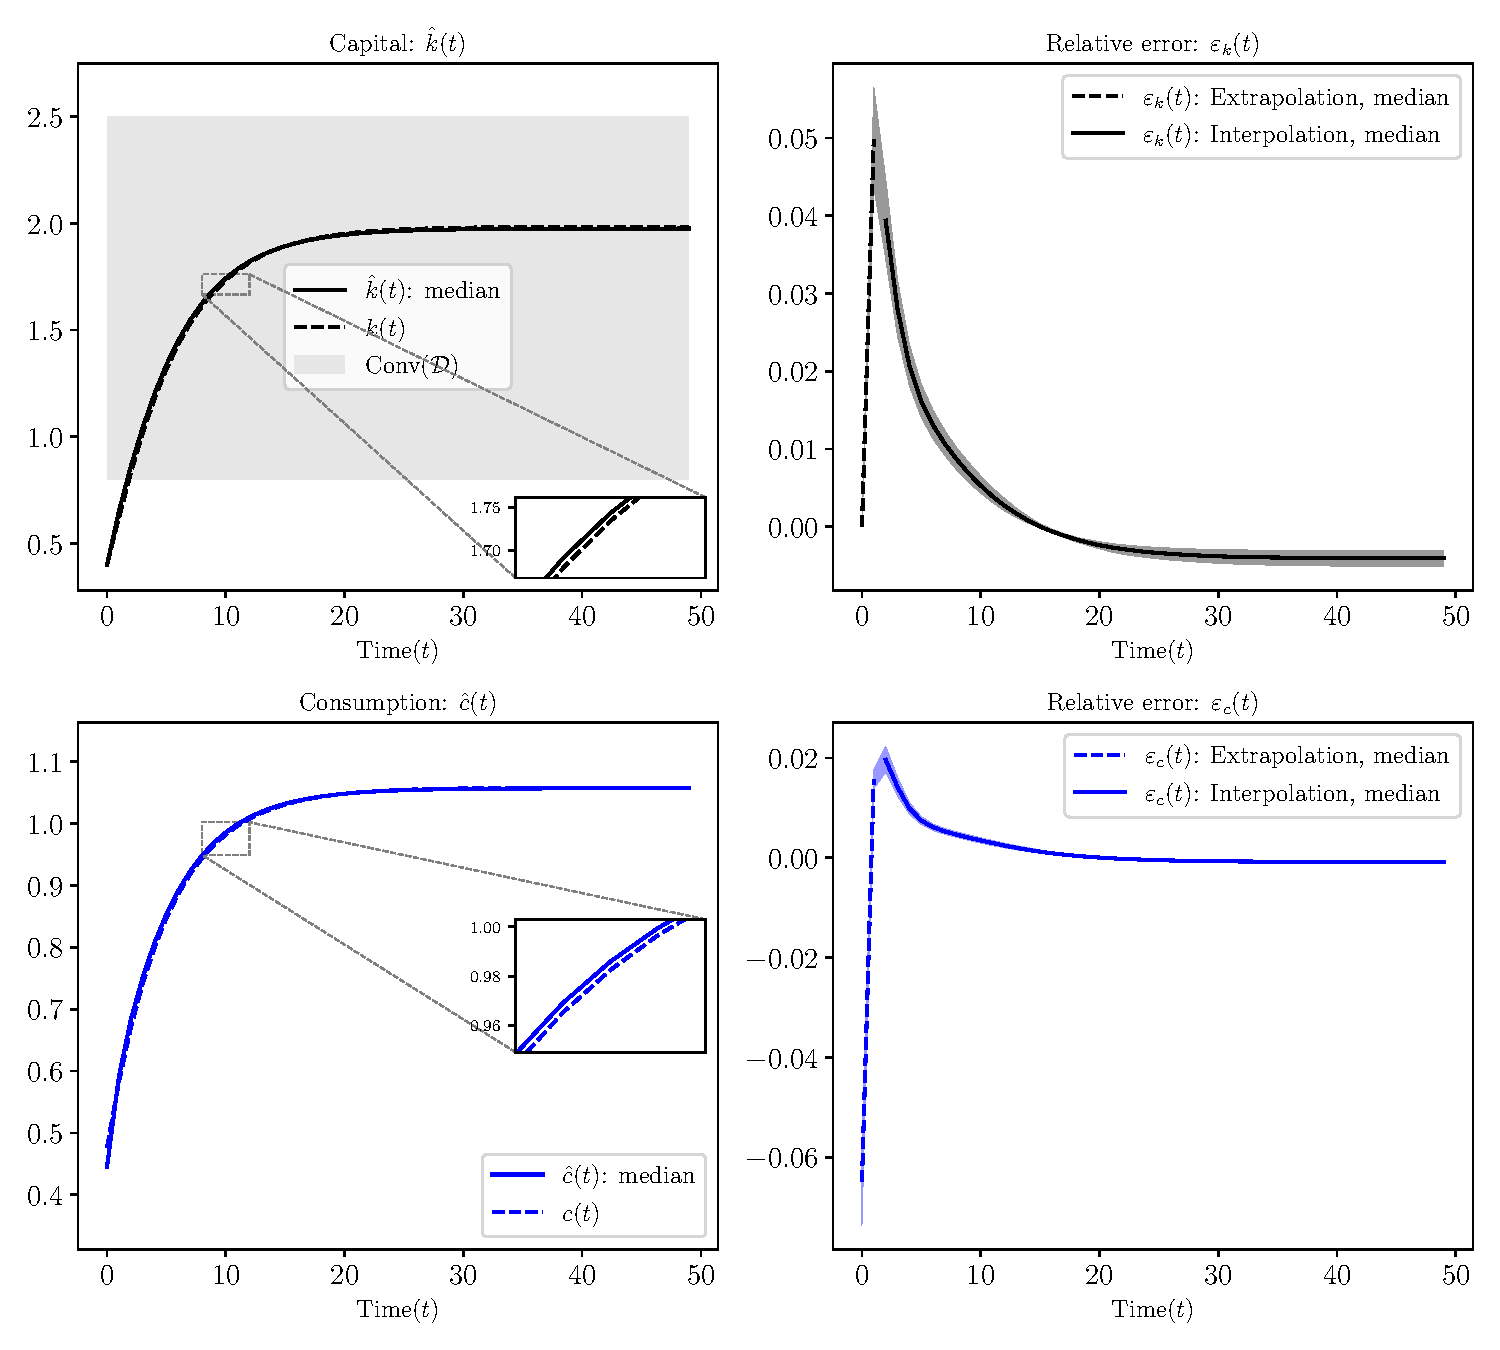
\includegraphics[width= 8cm]{figs/growth_recursive_g0_ensemble.pdf}}
		%\includegraphics[width=8cm]
	\end{minipage}
	\hfill%
	\begin{minipage}[t]{0.5\textwidth}\raggedleft
		\begin{itemize}
			\item Picking $\mathcal{D} =[0.8,2.5]\times \{1\}$ and $k_0= 0.4 \not\in \mathcal{D}$ is ``extrapolation''  $\alpha=\frac{1}{3}$, $\sigma =1$, $\beta = 0.9$, and $g = 0$.
			\smallskip.
			\item Low generalization errors, even without imposing transversality condition.
			\item Results for $100$ different seeds (initialization of the parameters)
		\end{itemize}
		\hyperlink{rec-all-over-space}{\beamerskipbutton{For all $k\in \mathcal{D}$}}		
	\end{minipage}
\end{frame}

\begin{frame}{Far from the steady state}
	\begin{minipage}[t]{0.4\textwidth}
		\raisebox{-\height+0.7\baselineskip}{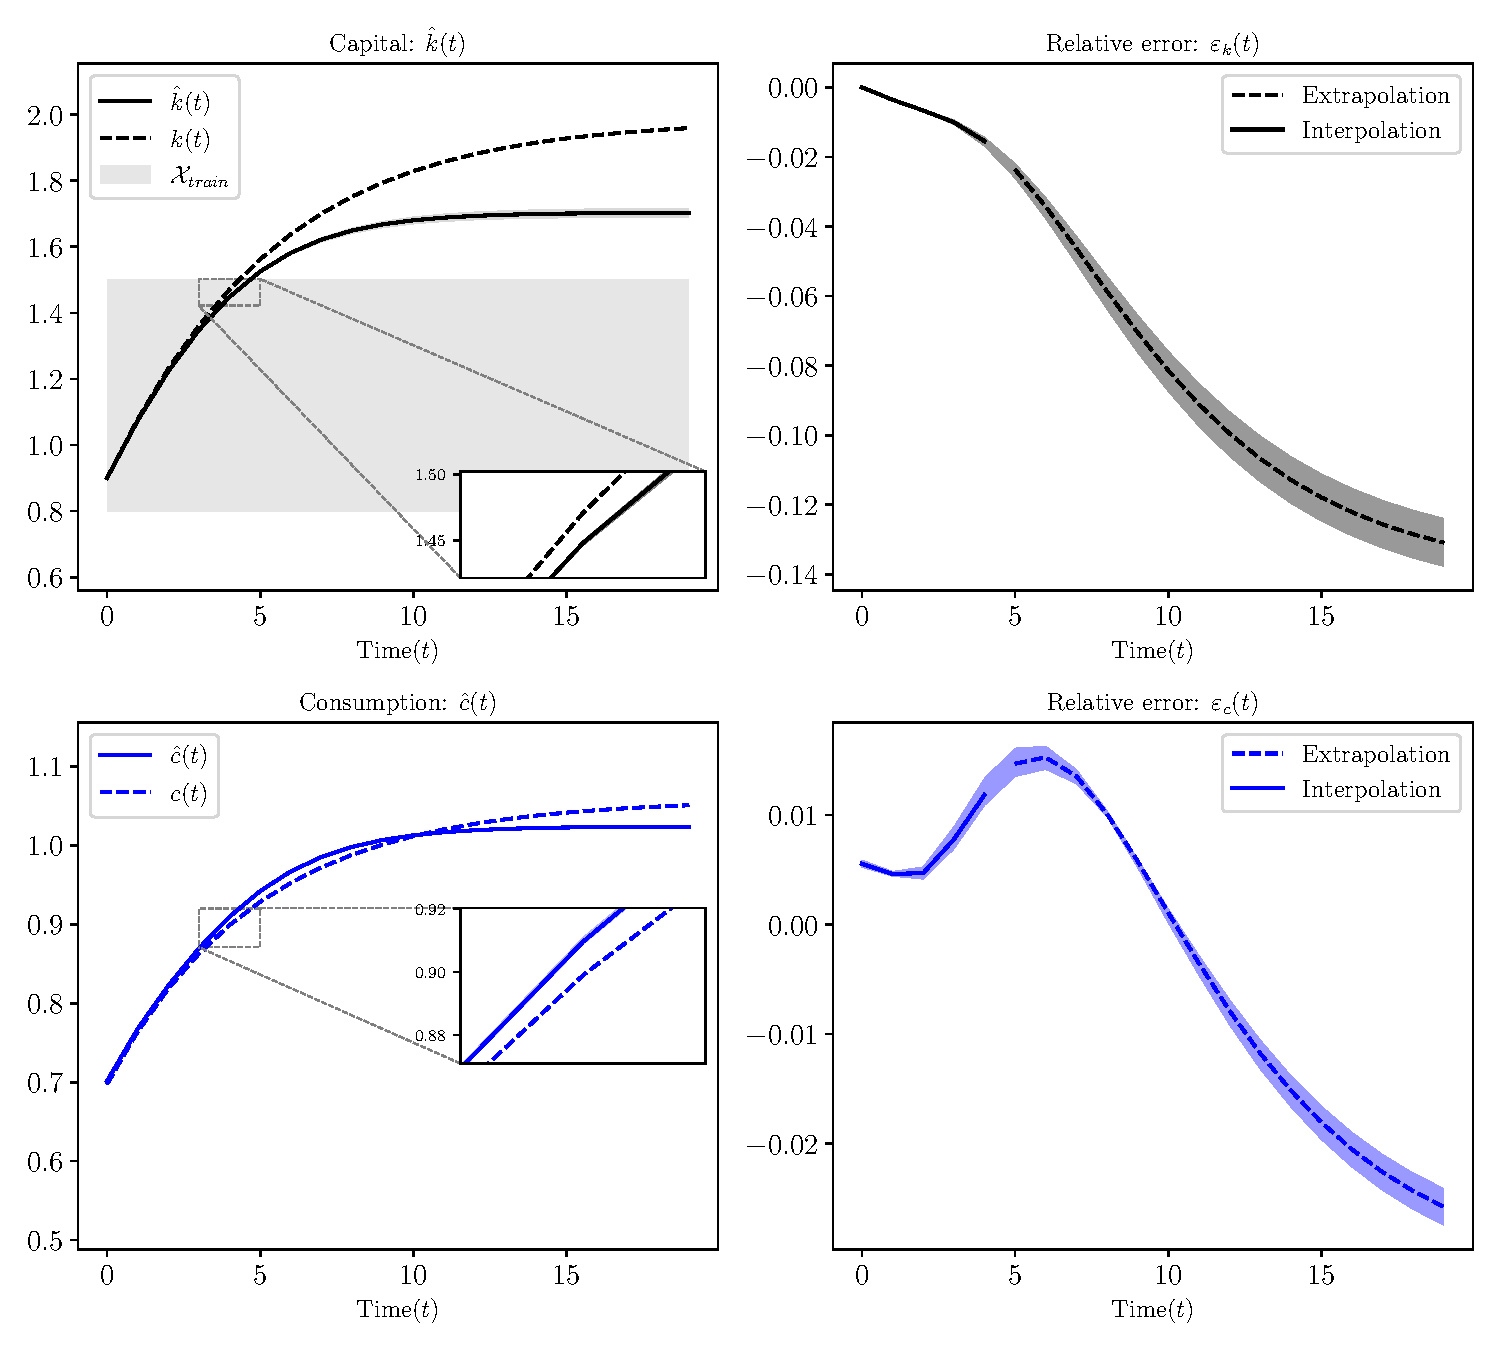
\includegraphics[width= 8cm]{figs/growth_recursive_g0_far_from_steady_state_ensemble.pdf}}
		%\includegraphics[width=8cm]
	\end{minipage}
	\hfill%
	\begin{minipage}[t]{0.5\textwidth}\raggedleft
		\begin{itemize}
			\item Picking $\mathcal{D}= [0.8,1.5]$ , $k^*\notin [0.8,1.5]$.
			\smallskip 
			\item A local grid around the $k_0$ is enough.   
			\begin{itemize}
				\item Accurate solutions in the interpolation region.
			\end{itemize}
			\smallskip 
			\item Generalization errors are not bad.
			\smallskip
			\item Results for $100$ different seeds (initialization of the parameters)
		\end{itemize}
	\end{minipage} 
\end{frame}

\begin{frame}[label = ncg_reg_growth_res]{Growing TFP}
	\begin{minipage}[t]{0.4\textwidth}
		\raisebox{-\height+0.7\baselineskip}{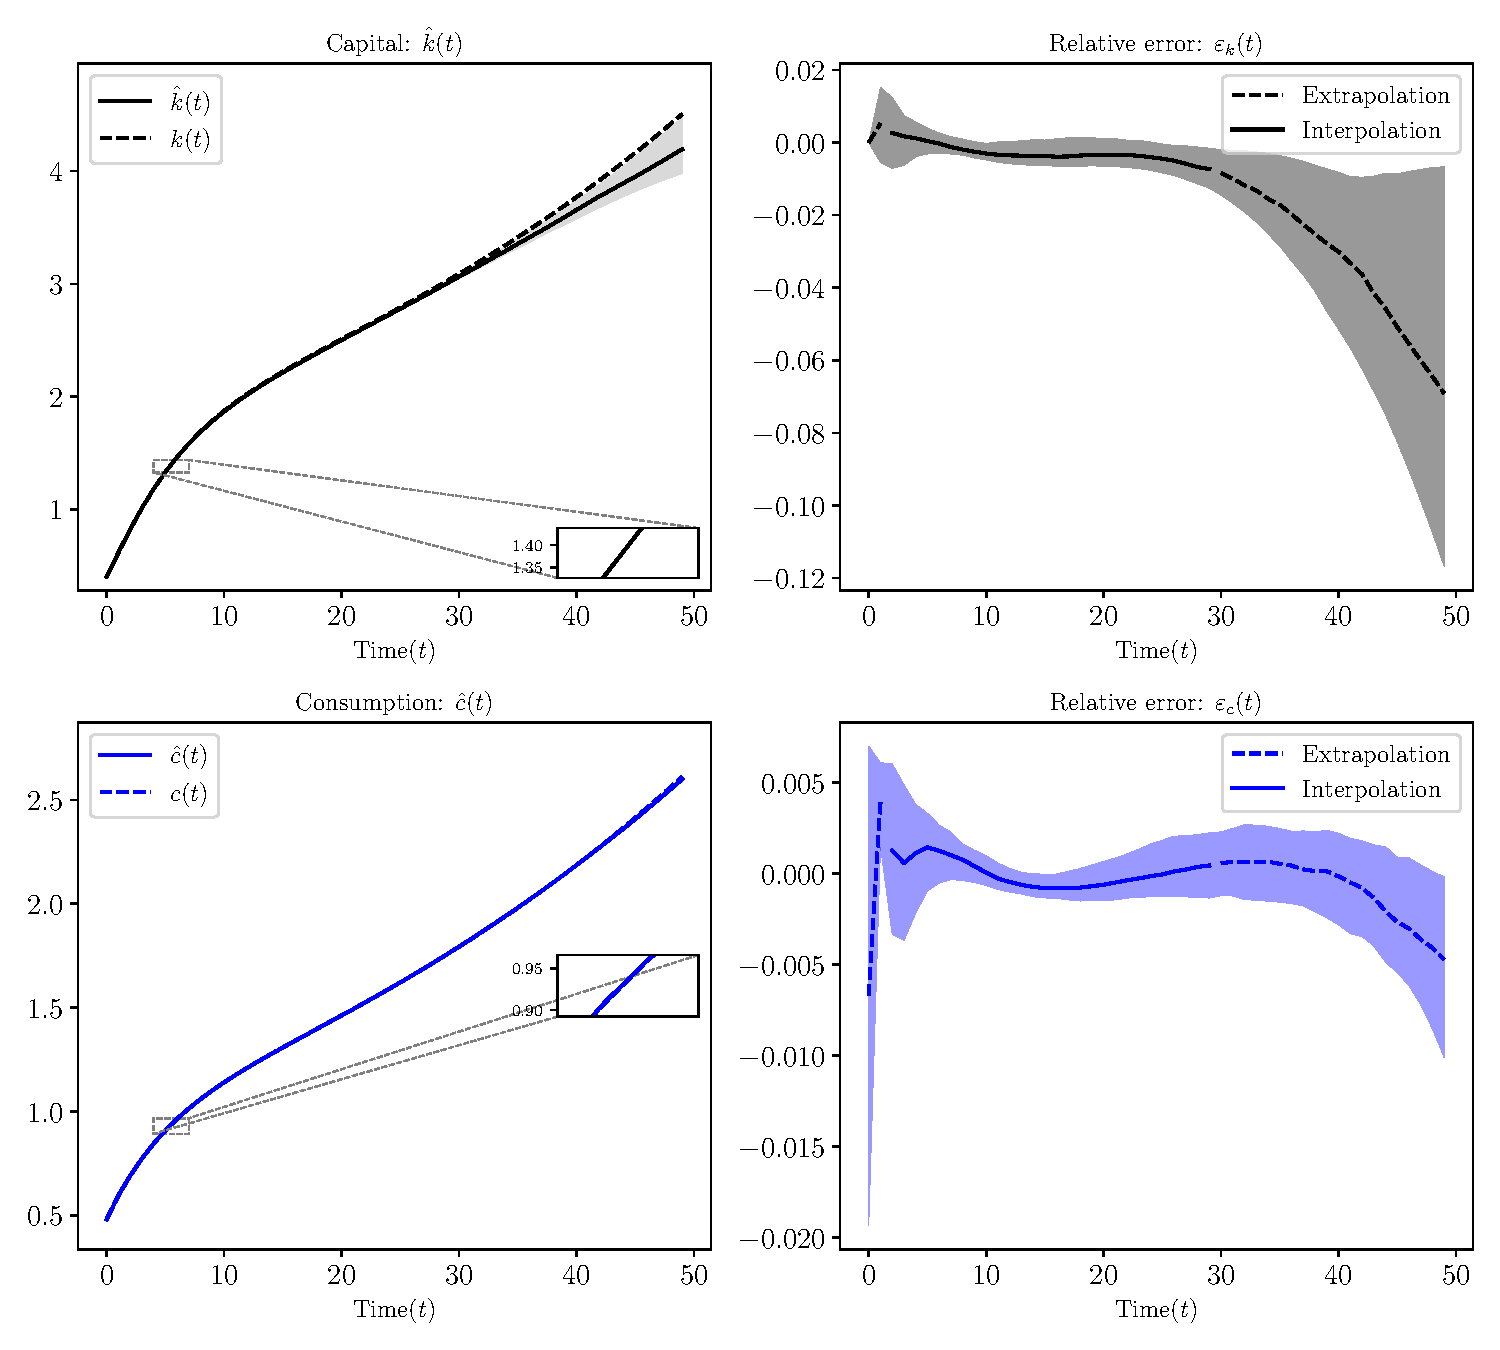
\includegraphics[width= 8cm]{figs/growth_recursive_g_positive_ensemble.pdf}}
		%\includegraphics[width=8cm]
	\end{minipage}
	\hfill%
	\begin{minipage}[t]{0.5\textwidth}\raggedleft
		\begin{itemize}
			\item Picking $\mathcal{D} = [0.8,3.5]\times[0.8,1.8]$ but now $g = 0.02$.
			\smallskip
			\item Choosing $k'(k,z;\theta) = z NN(\frac{k}{z},z;\theta)$.
			\begin{itemize}
				\item Here we used economic intuition to design the $\mathcal{H}(\Theta)$.
			\end{itemize}
			\smallskip
			\item Relative errors are very small inside the grid.
			\smallskip	
			\item  Small generalization errors.
		\end{itemize}
	\end{minipage}
\end{frame}

\section{Are Euler and Bellman residuals enough?}


\begin{frame}{Euler residuals are not enough}
	\begin{itemize}
		\item We picked a grid $\mathcal{D}$ and approximated $k'(k)$ with an over-parameterized function.			\smallskip
		\begin{itemize}
			\item The approximate solutions do not violate the transversality condition. 
		\end{itemize} 
		\smallskip
		\item What happens if we approximate the consumption functions $c(k)$ with an over-parameterized function.			\smallskip
		\begin{itemize}
			\item We get an interpolating solution, i.e, very small Euler residuals.			\smallskip
			\item However, the solutions \emphcolor{violate} the transversality condition. 			\smallskip
		\end{itemize}
	\end{itemize}
	
	\emphcolor{Intuition:}  consumption functions with low derivatives leads to optimal policies for capital with big derivatives.
\end{frame}


\begin{frame}{Small Euler residuals can be misleading}
	\begin{minipage}[t]{0.4\textwidth}
		\raisebox{-\height+0.7\baselineskip}{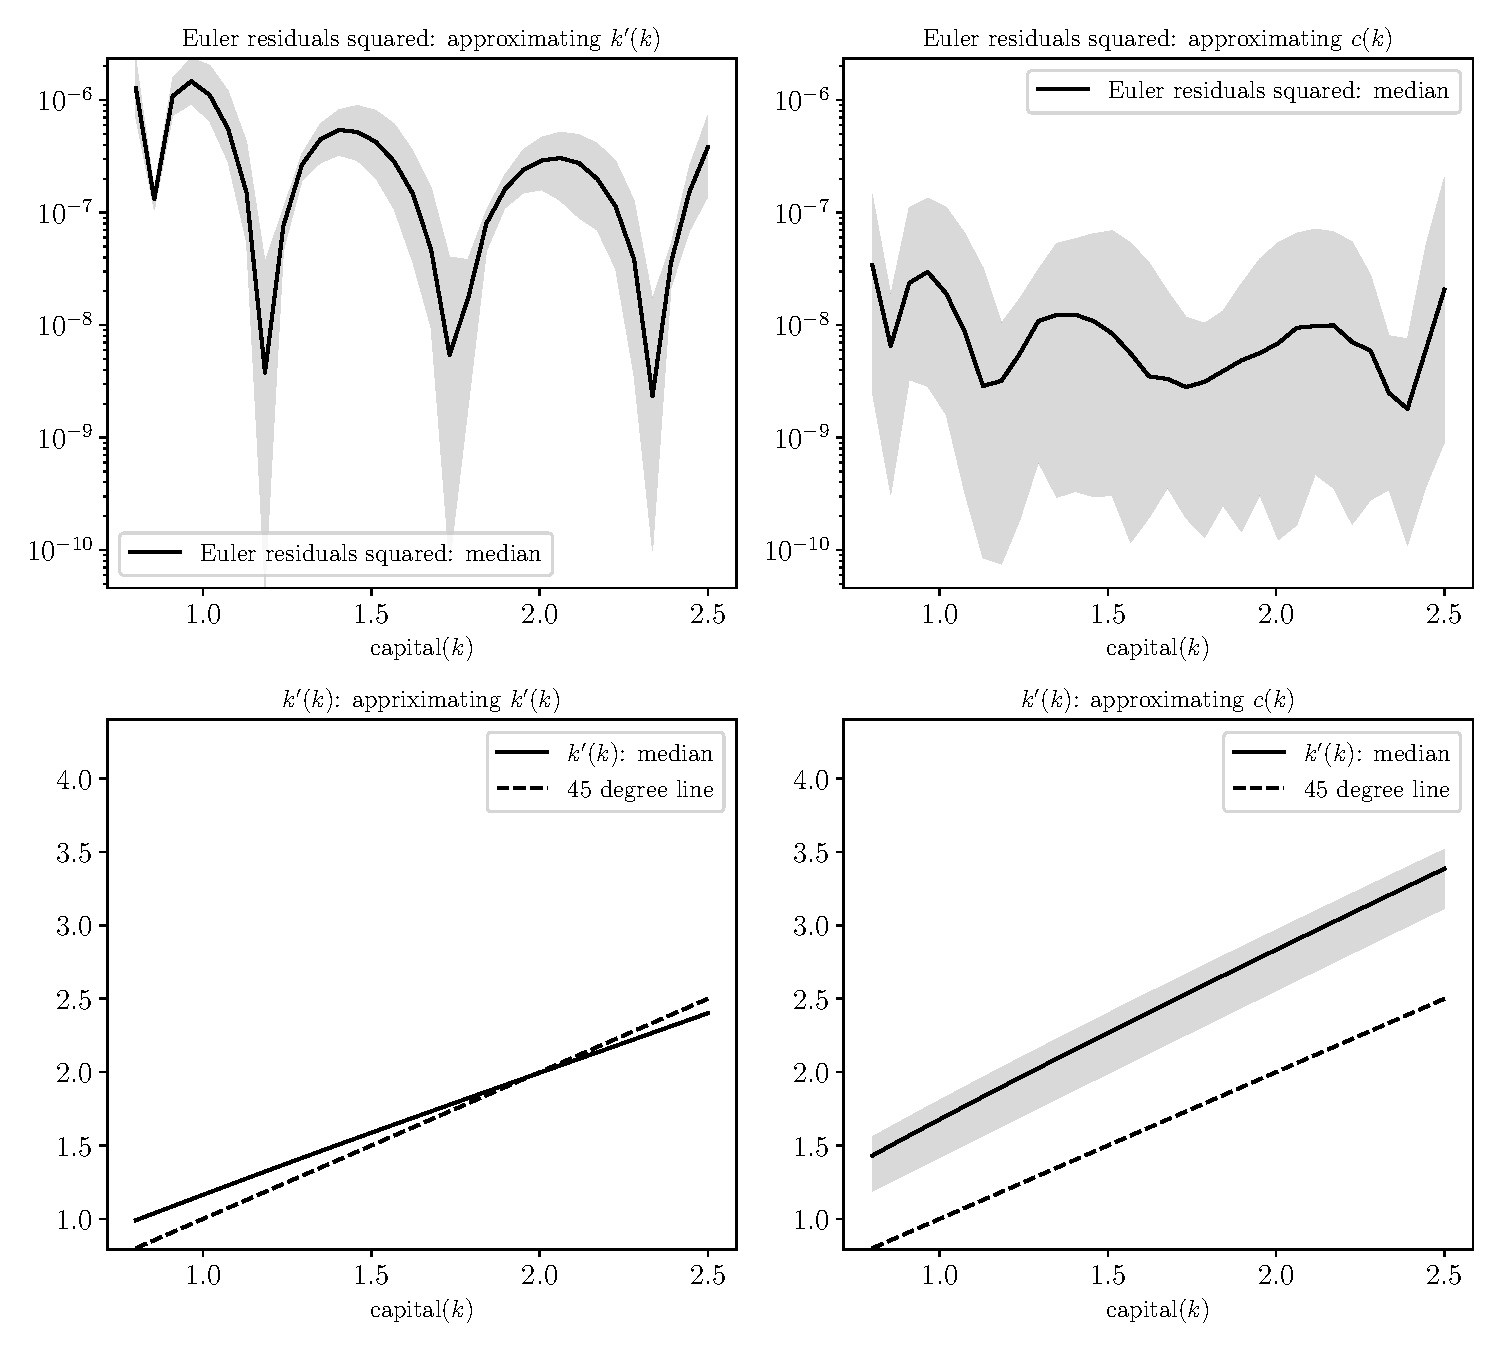
\includegraphics[width= 8cm]{figs/growth_recursive_g0_euler_residuals_grid.pdf}}
	\end{minipage}
	\hfill%
	\begin{minipage}[t]{0.5\textwidth}\raggedleft
		\begin{itemize}
			\item Left panels: approximating $k'(k)$ with a deep neural network.			\smallskip
			\begin{itemize}
				\item The solutions do not violate the TVC.			\smallskip
				\item $k'(k)$ intersects with $45^{\circ}$ line at $k^*\approx 2$.			\smallskip
			\end{itemize}
			\smallskip
			\item Right panels: approximating $c(k)$ with a deep neural network.
			\begin{itemize}
				\item The solutions \emphcolor{violate} the TVC.			\smallskip
				\item $k'(k)$ intersects with $45^{\circ}$ line at $\tilde{k}_{\text{max}}\approx 30$.			\smallskip
				\item Euler residuals are systematically lower. 
			\end{itemize}
			
		\end{itemize}
	\end{minipage}
\end{frame}


\begin{frame}{Can regularization fix this problem?}
	\begin{minipage}[t]{0.4\textwidth}
		\raisebox{-\height+0.7\baselineskip}{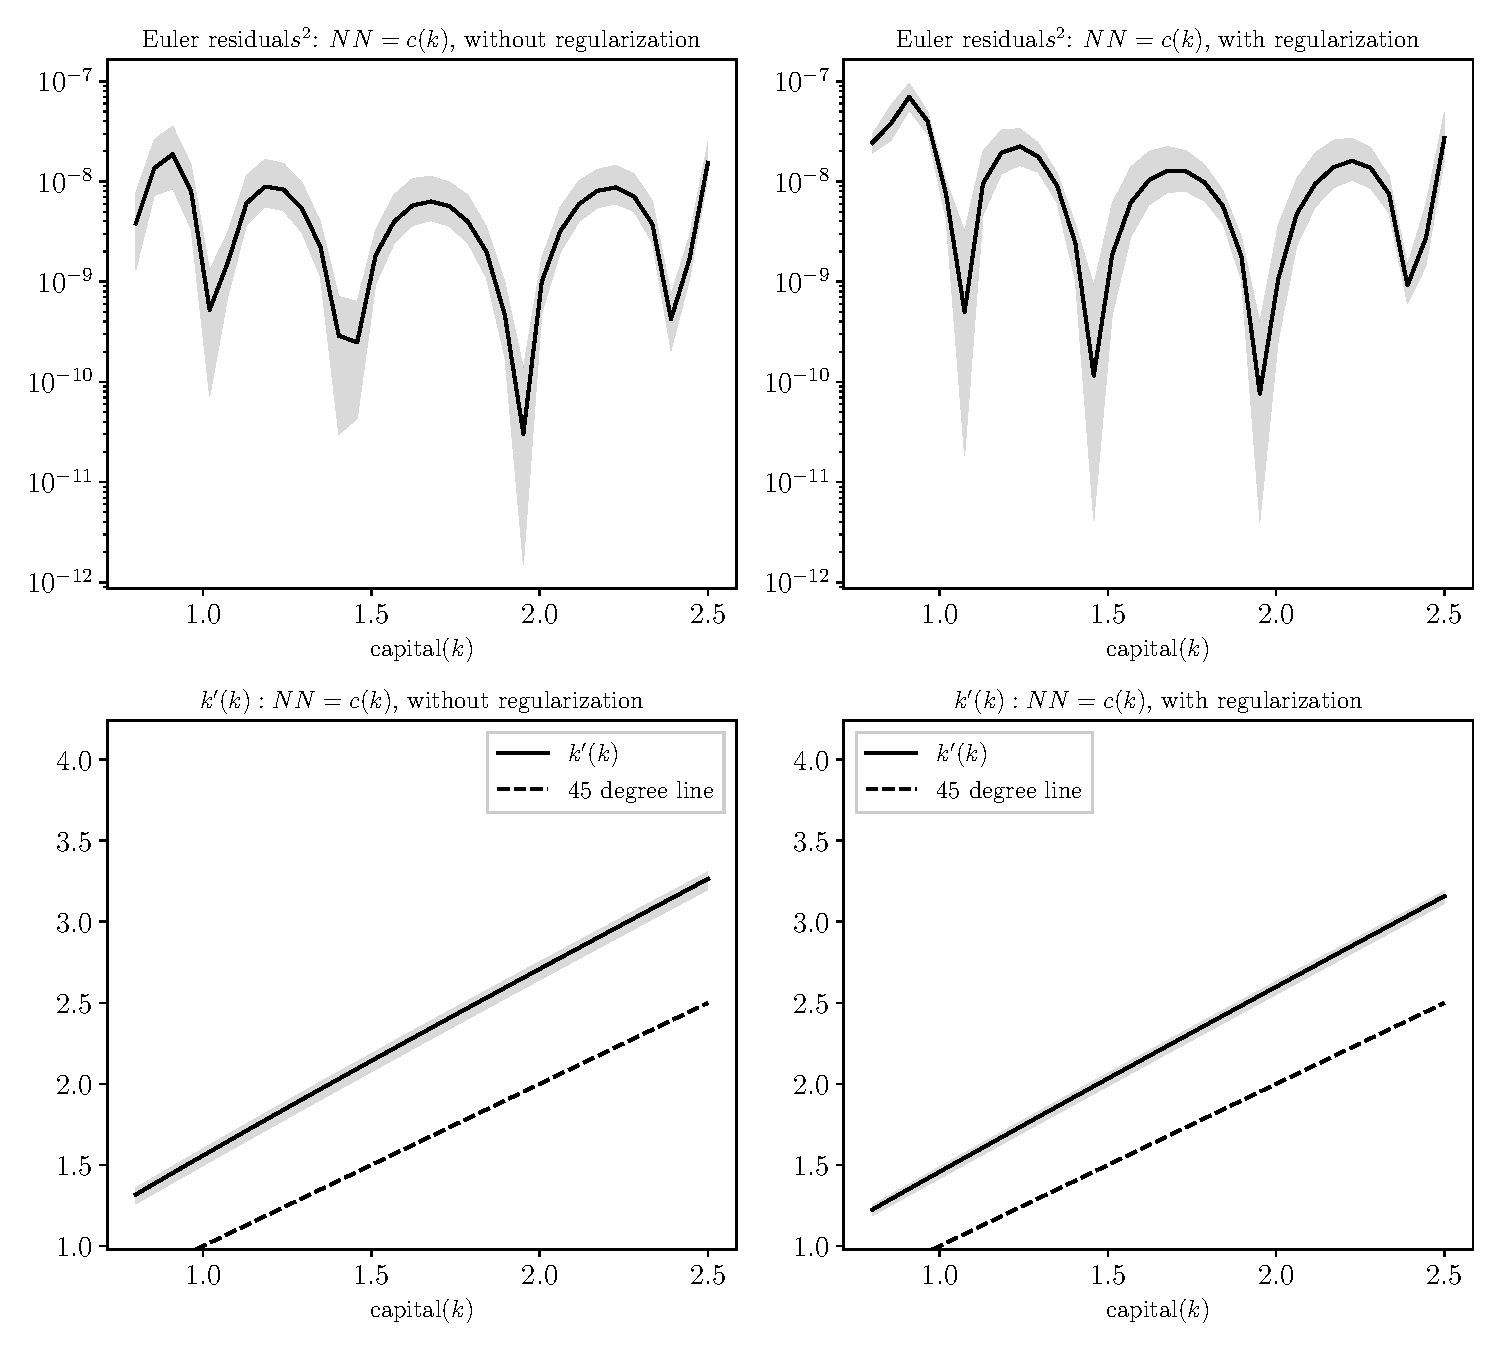
\includegraphics[width= 8cm]{figs/growth_recursive_g0_euler_residuals_grid_reg.pdf}}
	\end{minipage}
	\hfill%
	\begin{minipage}[t]{0.5\textwidth}\raggedleft
		\begin{itemize}
			\item Left panels: approximating $c(k)$ with a deep neural network without explicit regularization.			\smallskip
			\item What does happen with $L_2$ regularization?
			\smallskip
			\begin{itemize}
				\item Penalizing $\sum_{\theta_i \in \Theta} \theta_i^2$.
			\end{itemize}
			\item Right panels: approximating $c(k)$ with a deep neural network \emphcolor{with} explicit regularization.\smallskip
			\item Using deep learning requires understanding the \emphcolor{inductive bias} and \emphcolor{economic theory}.
		\end{itemize}
	\end{minipage}
\end{frame}






\begin{frame}{Conclusion}
	\begin{itemize}
		\item Short- and medium-run accurate solutions can be obtained \emphcolor{without} strictly enforcing the long-run boundary  conditions on the model’s dynamics.
		\vspace{0.1in}
		\item Long-run (\emphcolor{global}) conditions can be replaced with appropriate regularization (\emphcolor{local}) to achieve optimal solutions, hence the title of the paper.
		\vspace{0.1in}
		\item Inductive bias provides a foundation for modeling forward-looking behavioral agents with self-consistent expectations.
	\end{itemize}
\end{frame}

\begin{frame}{Discussion: where to go from here?}
	\begin{itemize}
		\item Can inductive bias/regularization be thought of as an equilibrium selection device?
		\begin{itemize}
			\item In this paper it is used to select solutions.
		\end{itemize}
		\smallskip
		\item This method (mostly the kernel method) can be used for sampling high-dimensional state spaces when there is stochasticity. 
		\begin{itemize}
		\item Solve the deterministic in short-run and use the points as sample of the state-space.
		\smallskip
		\item Then solve the stochastic problem.
		\end{itemize}
		%if we are about to translate economic dynamic models into an ERM, can regularization act as an equilibrium device? Think about it, ERM in statistical learning or machine learning is about two things: uniform of law of large numbers and capacity control (so what are going to do about this capacity control regularization)
	\end{itemize}
\end{frame}

\section{Appendix}

\begin{frame}{Deep Learning: random initialization and non-convex optimization  }
\label{dif_dist}
	
	\begin{figure}[t!]
		\centering
		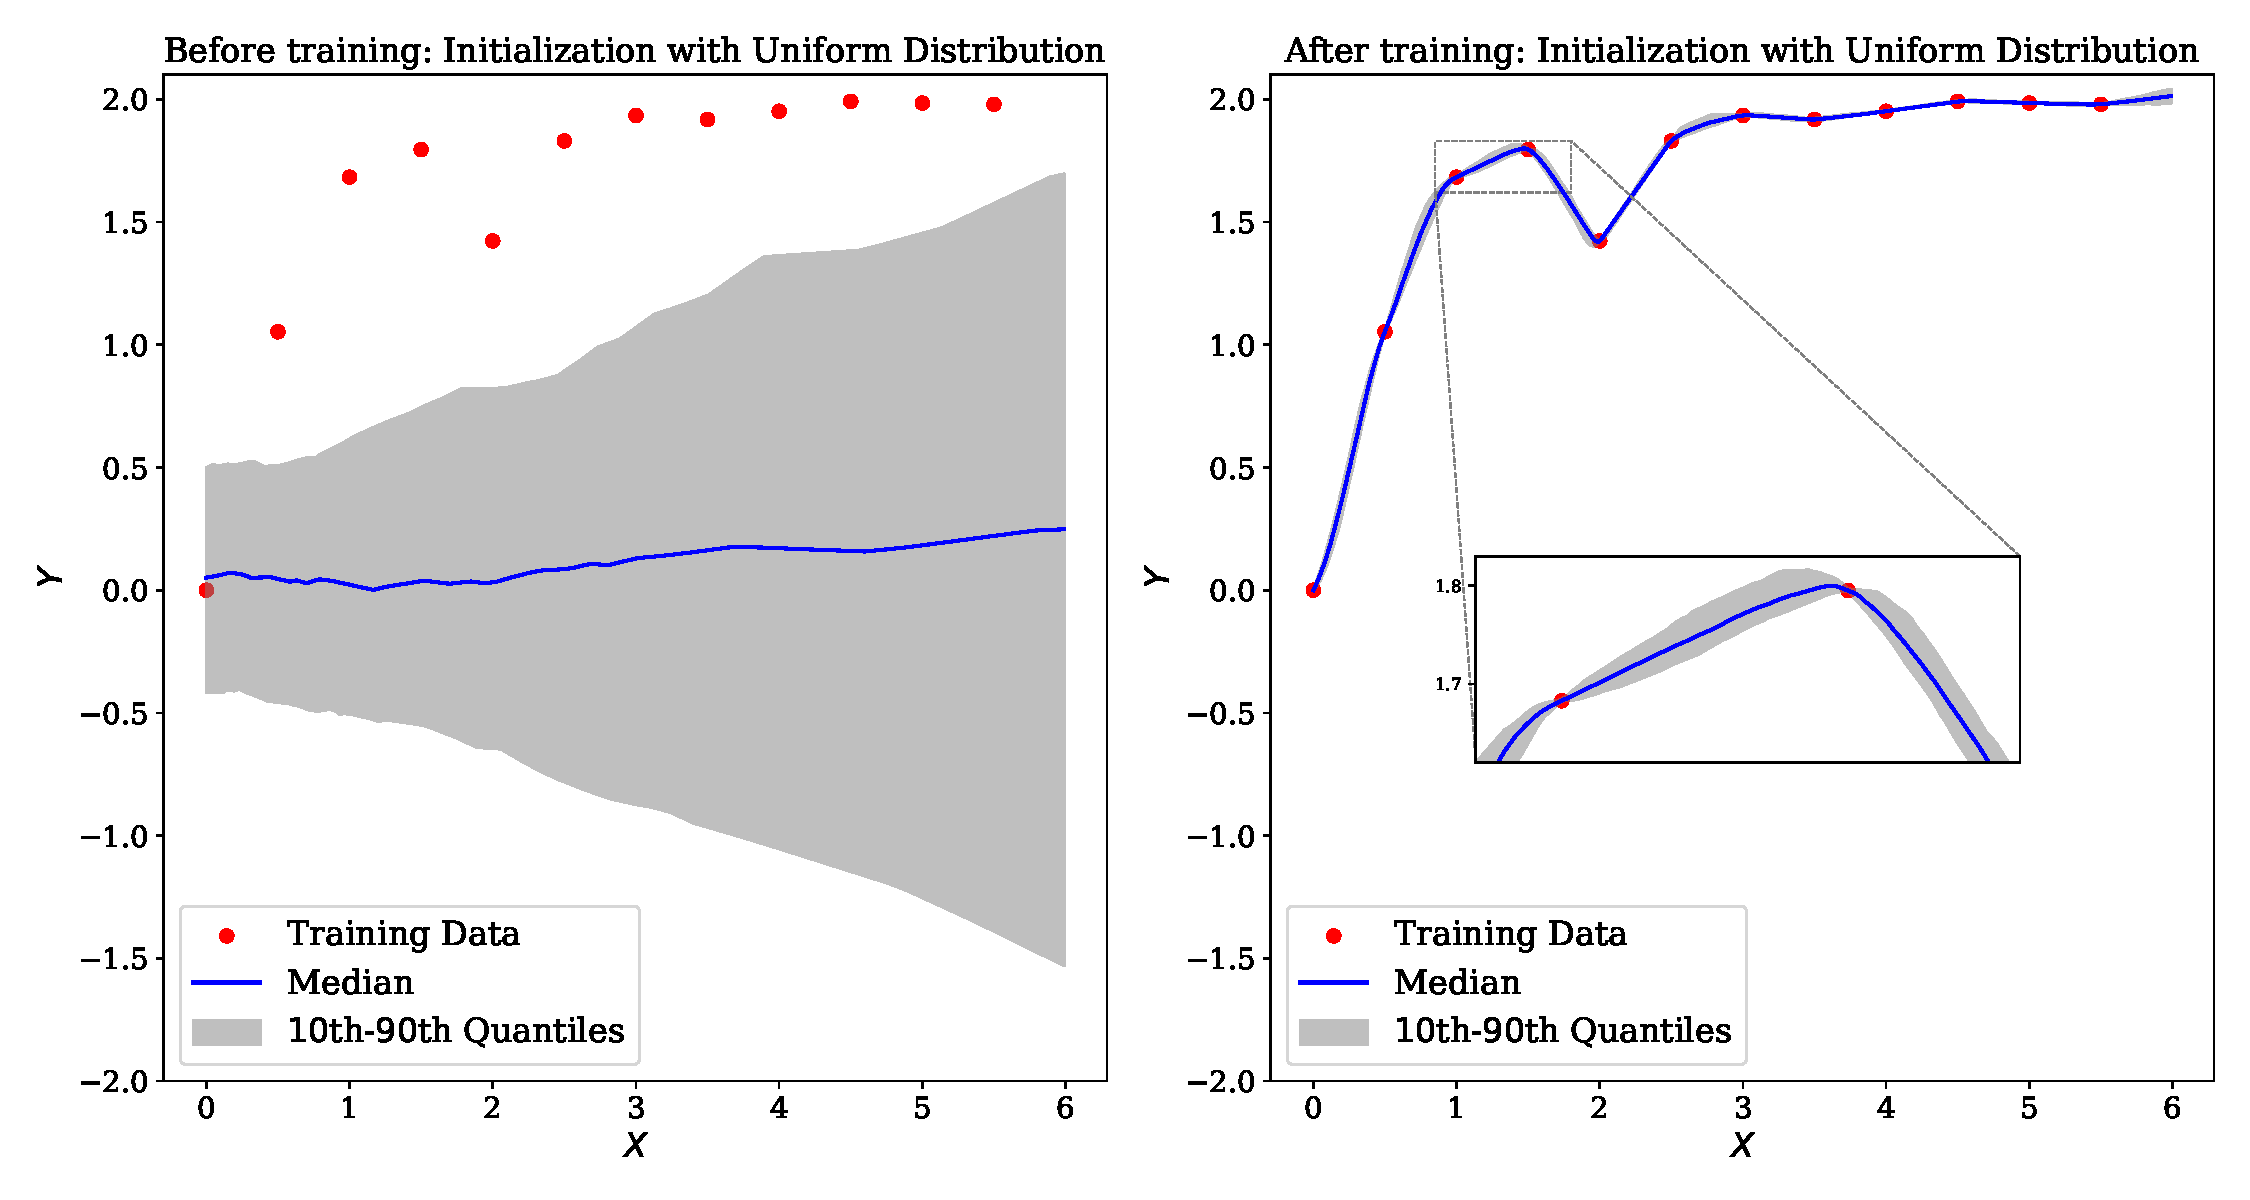
\includegraphics[width=0.75\textwidth]{figs/smooth_interpolation_100_seeds_uniform_init.pdf}
	\end{figure}
	%The parameters are irrelevant
	% RelU, 3 layers, Adam optimizer
	\hyperlink{non_convex}{\beamerskipbutton{Back}}
	%Four layer neural networks, with ReLU activation, 128 nodes
	%init.uniform_(self.y[0].weight, a=-0.25, b=0.25)  
	%init.uniform_(self.y[0].bias, a=-0.25, b=0.25)    
\end{frame}


\begin{frame}[label = rec-all-over-space]
	\frametitle{Results: initial conditions over the state space}
	\begin{figure}[t!]
		\hspace*{-15mm}
		\centering
		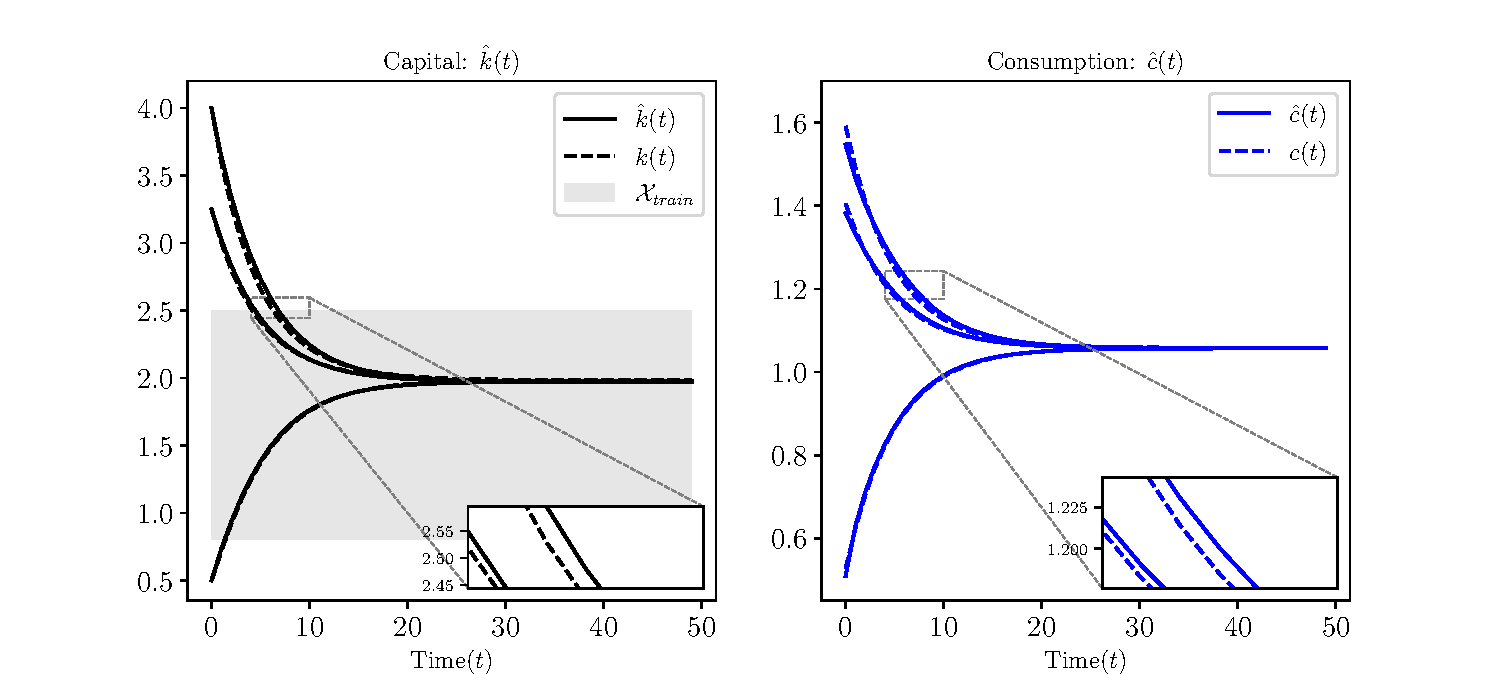
\includegraphics[width=0.7\textwidth]{figs/growth_recursive_g0_var_initial_k_0_one_run}
	\end{figure}
		\begin{itemize}
			\item The solution has to satisfy the transversality condition for all points in $\Xdom$ 			\smallskip
			 $\lim_{T\to\infty}\beta^T u'(c(T))k(T+1) =0 \quad \forall ~ k_0 \in \Xdom$
			 \item Three different initial condition for capital, all outside of $\Xdom$.
		\end{itemize}
		\hyperlink{res-rec}{\beamerskipbutton{back}}
\end{frame}



\end{document}
